\chapter{Herramienta}

El entrenamiento de modelos de representaciones vectoriales es un proceso costoso tanto desde el
punto de vista computacional como cognitivo: requiere recopilar una gran cantidad de texto,
realizarle un preprocesamiento adecuado (e.g.\ sacarle mayúsculas, símbolos), utilizarlo para
alimentar a un modelo que tiene un gran consumo de memoria y de poder de cómputo, para luego obtener
un modelo vectorial también de gran tamaño. Este modelo debe también poder evaluarse para determinar
su utilidad, corriendo una variada batería de pruebas, explorando así el espacio de hiperparámetros
para obtener una configuración razonable.

Con el fin de simplificar este proceso, y permitir a cualquier investigador realizar experimentos
con modelos vectoriales, se plantea la elaboración de una herramienta que sea capaz de abstraerse de
todas las tareas de bajo nivel, permitiendo construir representaciones vectoriales a través de una
interfaz web. El objetivo es pues brindar una herramienta que, en base a un fragmento del corpus y
una configuración de hiperparámetros, entrene y deje disponible para utilizar vectores de palabras
generados a medida para una tarea particular.


\section{Requerimientos}

Antes de iniciar la construcción de la herramienta, se fijaron una serie de requerimientos que se
esperaba que la misma lograra satisfacer:

\begin{itemize}

\item Dado que se cuenta con un corpus de gran tamaño, etiquetado y almacenado en un motor de
búsqueda, es conveniente ofrecer la posibilidad de explorarlo de manera interactiva. Para esto se
pretende brindar funcionalidades de búsqueda a través de consultas de texto basadas en el contenido
de los documentos, o filtrando a partir de los campos estructurados (los metadatos, la fuente de
palabras, las etiquetas, etc.).

Esto permitirá que un usuario pueda encontrar ejemplos particulares de uso del lenguaje fácilmente
pudiendo, por ejemplo, ver todos los documentos donde aparece la palabra \textit{fútbol} en portales
de noticias Uruguayos (documentos con las etiquetas \textit{uruguay} y \textit{news}). Lograr
particionar así el corpus permitirá también entrenar vectores con datos especializados.

\item Los algoritmos que se utilizan para construir representaciones vectoriales requieren de una
capacidad de cómputo muy elevada, por lo que no se pueden entrenar localmente en una computadora
común (al menos no en tiempos razonables). Por esta razón, es imprescindible contar con un servidor
de cómputo especializado que tenga las capacidades necesarias para correr los algoritmos.

Resulta conveniente, por lo tanto, que la interfaz sirva de mediador entre el usuario y dicho
servidor, pudiendo entrenar o evaluar modelos allí de manera remota, para no tener que realizar esta
tarea manualmente, que presenta sus dificultades. Así, un usuario será capaz de enviar a entrenar un
modelo y que éste quede corriendo de fondo en el servidor de cómputo por el tiempo que sea
necesario, sin requerir de interacción adicional hasta que el algoritmo finalice.

\item Además de brindar acceso a un servidor especializado, se desea que el usuario pueda entrenar
los algoritmos deseados a medida, a partir del corpus o de secciones del mismo. Para ello, deberá
ser posible elegir el modelo de representación vectorial a utilizar (Skipgram, CBOW, GloVe, o PPMI),
junto a los hiperparámetros que cada uno de ellos posee. Además es necesario que se pueda indicar
qué corpus utilizar para el entrenamiento, pudiendo elegirse la totalidad del mismo o secciones
particulares en caso que se desee obtener vectores especializados en algún campo. Para esto último,
se deberá permitir ingresar una consulta de Elasticsearch para usar el resultado de la misma como
corpus de entrenamiento.

\item También debe ser posible dar de alta conjuntos de pruebas para distintos tipos de tareas (esto
es, analogías, similitud entre palabras, etc.) y correr las evaluaciones en los modelos ya
entrenados, pudiendo estudiar así el comportamiento de los mismos en distintos escenarios.

\item Considerando estos dos últimos puntos, también es deseable que el usuario pueda fácilmente
visualizar y comparar el resultado obtenido en un conjunto de pruebas para los distintos modelos
entrenados, pudiendo así elegir fácilmente la mejor configuración de hiperparámetros para una tarea
particular.

\item Puesto que tanto el corpus como los modelos y los conjuntos de pruebas están almacenados en
servidores remotos, es necesario poder descargarlos. Para el corpus es deseable también ofrecer la
posibilidad de descargar partes del mismo para no tener que procesarlo localmente, lo cual puede ser
muy costoso debido a su tamaño.

\item Dado que el proceso de construcción del corpus es continuo, como se detalló en la sección de
scraping automático, puede ser de utilidad ofrecer estadísticas sobre la composición del mismo,
incluyendo cómo ha variado su tamaño recientemente, con el fin de poder controlar que el proceso
de extracción esté funcionando correctamente. Esto ayuda a detectar cuando una fuente de palabras
ha dejado de contribuir texto, lo cual puede ocurrir por, por ejemplo, un cambio en el diseño de la
misma que rompa las reglas XPath empleadas.

\item Por último, es importante tener en cuenta la usabilidad de la herramienta, manteniendo presente
que la misma debe facilitar la construcción de modelos vectoriales, y no dificultar la tarea. Para
esto, deberá prestarse especial cuidado al diseño final de la misma.

\end{itemize}

En definitiva, uno de los objetivos principales de la herramienta es la coordinación entre los
distintos componentes de la arquitectura de la aplicación. Se cuenta por un lado con un nodo
Elasticsearch donde se almacena de manera organizada todo el corpus recopilado. También se cuenta
con un servidor de cómputo que entrena y evalúa remotamente los modelos deseados. La herramienta
servirá como nexo para estos dos nodos, permitiendo al usuario acceder, interactuar y descargar los
distintos artefactos (corpus, modelos, pruebas) de la aplicación.


\section{Diseño de la Solución}

En esta sección se presenta el diseño de la herramienta a alto nivel. El objetivo principal aquí es
mostrar las funcionalidades principales de la misma desde el punto de vista de un usuario. La discusión
es por tanto a nivel conceptual, haciendo especial hincapié en mostrar qué puede hacerse con la herramienta
y cómo se organizan estas funcionalidades.

Desde el punto de vista conceptual, la herramienta se divide en cuatro grandes secciones:
\textit{Dashboard}, \textit{Corpus}, \textit{Embeddings} y \textit{Tests}. A continuación se encuentra la
descripción en detalle de cada una de estas secciones.

La solución aquí descrita puede ser accedida a través de la dirección\\
\href{http://golbat.ydns.eu}{http://golbat.ydns.eu}.

\subsection{Dashboard}

La sección \textit{Dashboard} es la más sencilla aunque aporta elementos de visualización muy útiles.
Principalmente se incluye un apartado por cada fuente utilizada para construir el corpus. En dichos
apartados se detalla el nombre de la fuente, la cantidad de palabras que la misma aporta al corpus y una
pequeña gráfica que muestra la cantidad de palabras que han sido obtenidas recientemente de dicha fuente.

\begin{figure}[h]
    \centering
    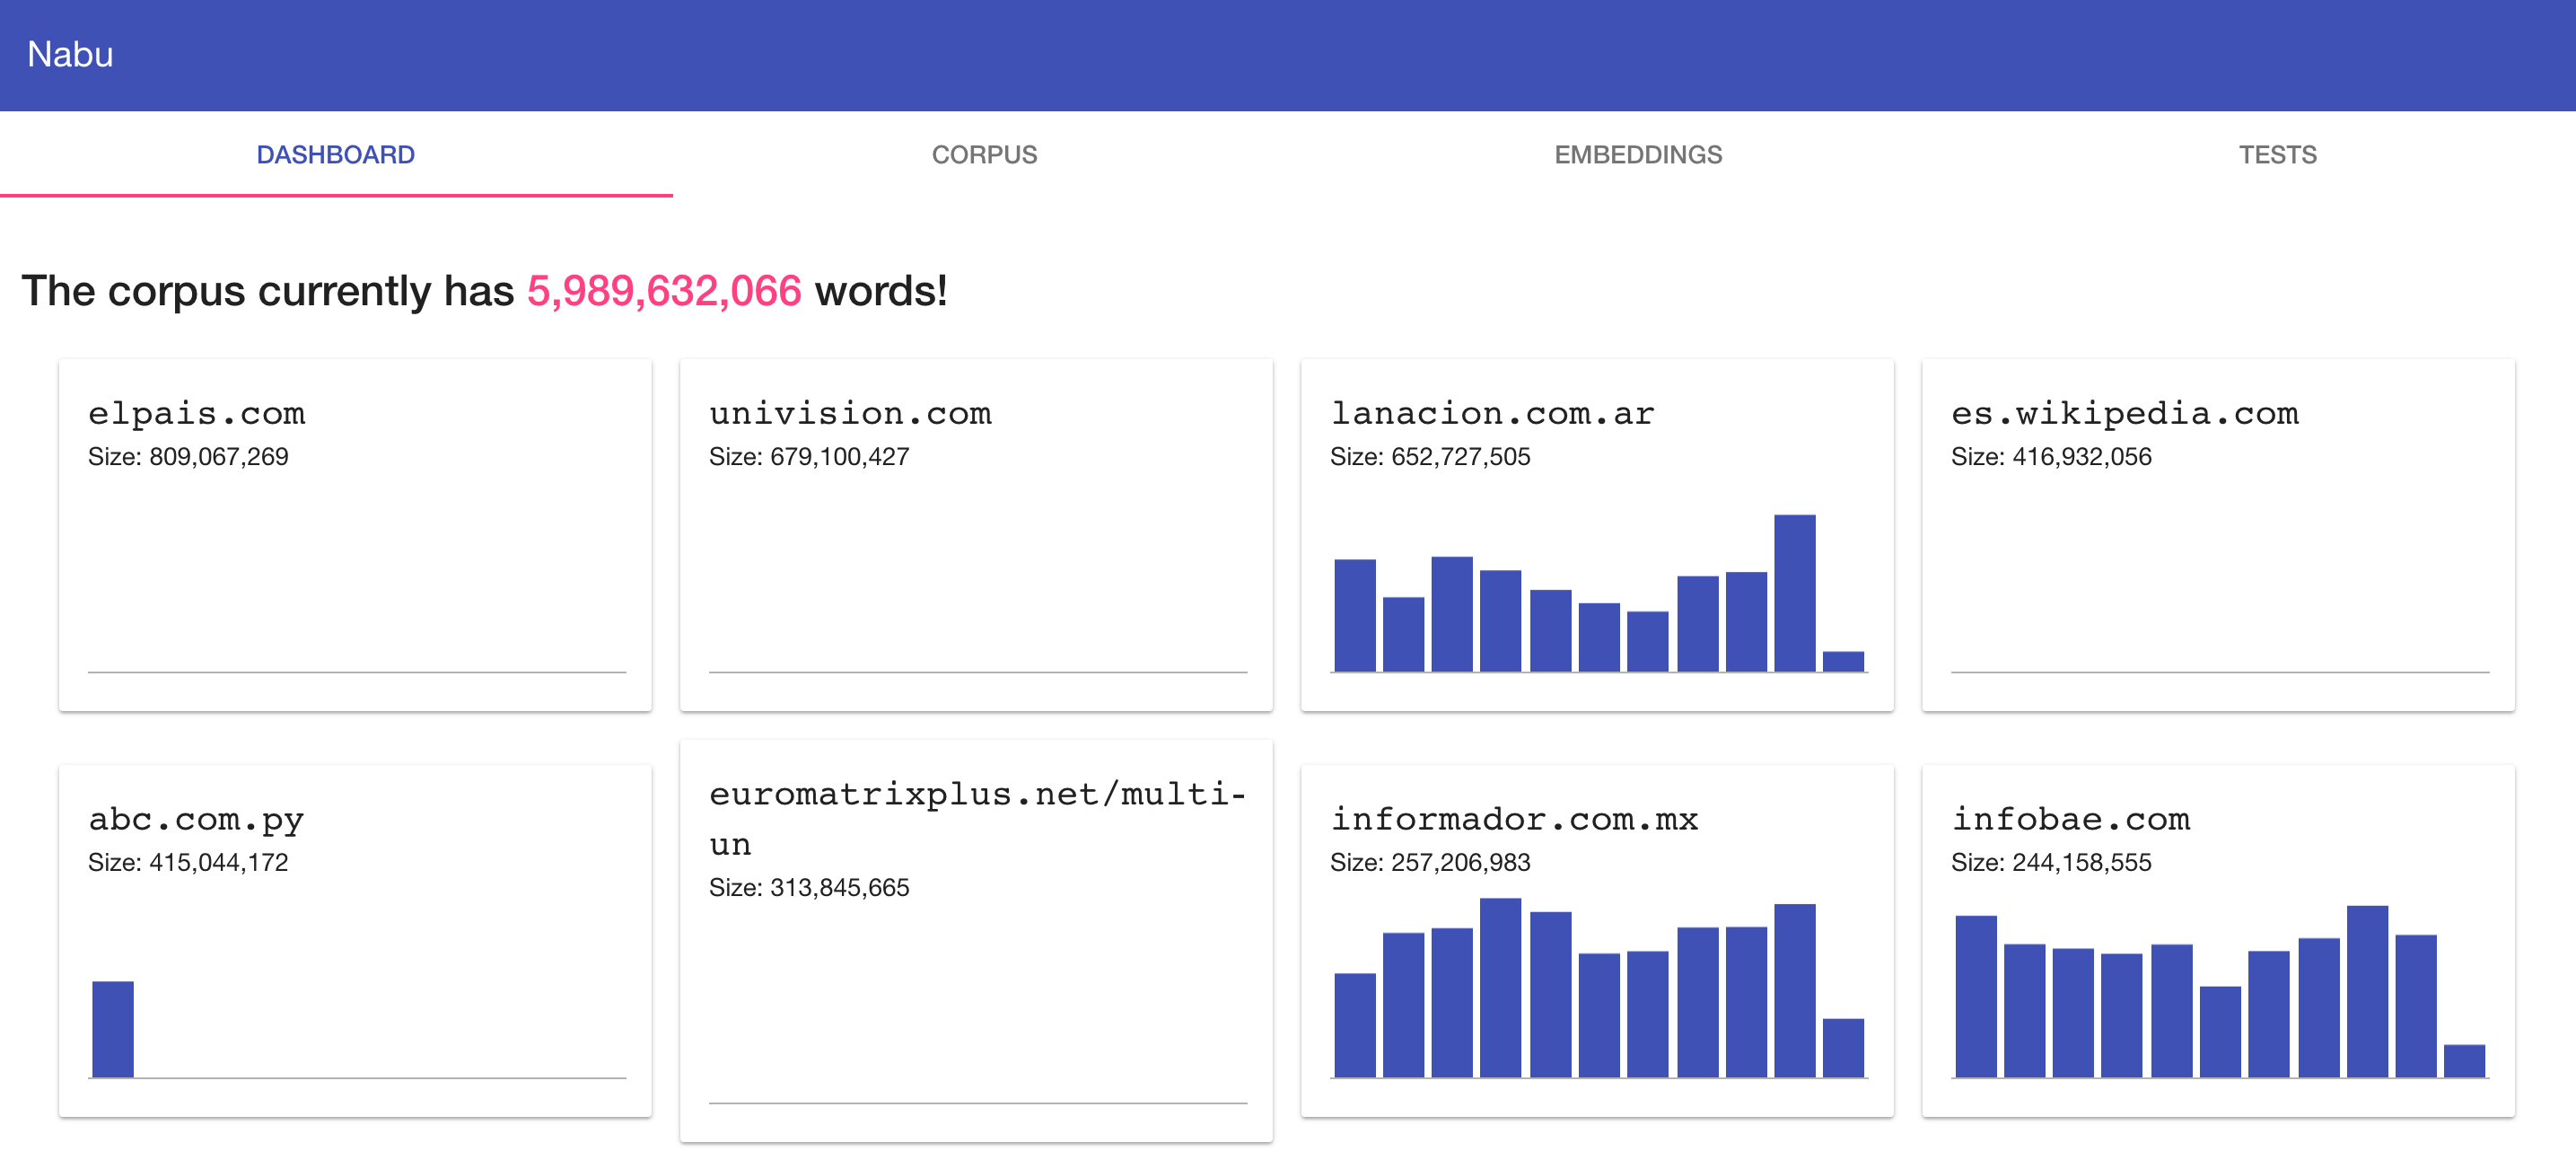
\includegraphics[width=\textwidth]{images/ui-nabu-dashboard}
    \caption{\textit{Pantalla Dashboard en la aplicación web.}}
    \label{fig:ui-nabu-dashboard}
\end{figure}

Estás gráficas cumplen la doble función de presentar la cantidad de palabras obtenidas de cada fuente de
forma diaria y además alertar de un posible defecto en el correspondiente script de extracción cuando la
cantidad extraída presenta una caída muy pronunciada con respecto a registros inmediatamente anteriores.

Como se explicó en secciones anteriores, fue necesario elaborar una cantidad considerable de scripts para
extraer información de las diferentes fuentes elegidas para construir el corpus. En algunos casos dicha
extracción se realizó en una única etapa. En otros casos, como por ejemplo los portales de noticias, es de
interés volver a visitar las fuentes de forma diaria para poder indexar los nuevos documentos que hayan
sido agregados. Naturalmente, las fuentes pueden cambiar su estructura y los scripts utilizados pueden
fallar ante estos cambios. Por este motivo, resulta sumamente útil contar con una forma visual de detectar
estos problemas rápidamente.

Finalmente, en esta sección se incluye la cantidad total de palabras que forman el corpus. Dicho número se
actualiza de forma automática en intervalos regulares y se despliega un mensaje cada vez que se obtienen
nuevas palabras de alguna de las fuentes.

\subsection{Corpus}

La sección \textit{Corpus} permite explorar la totalidad del corpus construido en el proyecto sin apenas
restricciones. Se ofrece un campo de búsqueda en el cual un usuario puede escribir una serie de términos
de consulta y se ofrece además la posibilidad de filtrar por un subconjunto de las fuentes consideradas.

Estas dos operaciones de apariencia sencilla construyen por detrás consultas en el formato JSON empleado
por Elasticsearch. Se permite visualizar y eventualmente modificar completamente la consulta inherente en
formato JSON a través del interruptor de \textit{consulta avanzada}. Al activar este interruptor, el
usuario cuenta con todo el poder de expresividad del formato de consultas de Elasticsearch y por tanto
puede ejecutar consultas potencialmente complejas sobre el corpus.

Una vez ejecutada una consulta se presenta una tabla con los documentos resultantes de la misma, con su
correspondiente paginación. En la tabla se incluye la fecha de extracción del documento, un breve fragmento
del texto que lo compone, resaltando los términos que lo hacen relevante a la consulta, y la fuente de la
que fue extraído.

\begin{figure}[h]
    \centering
    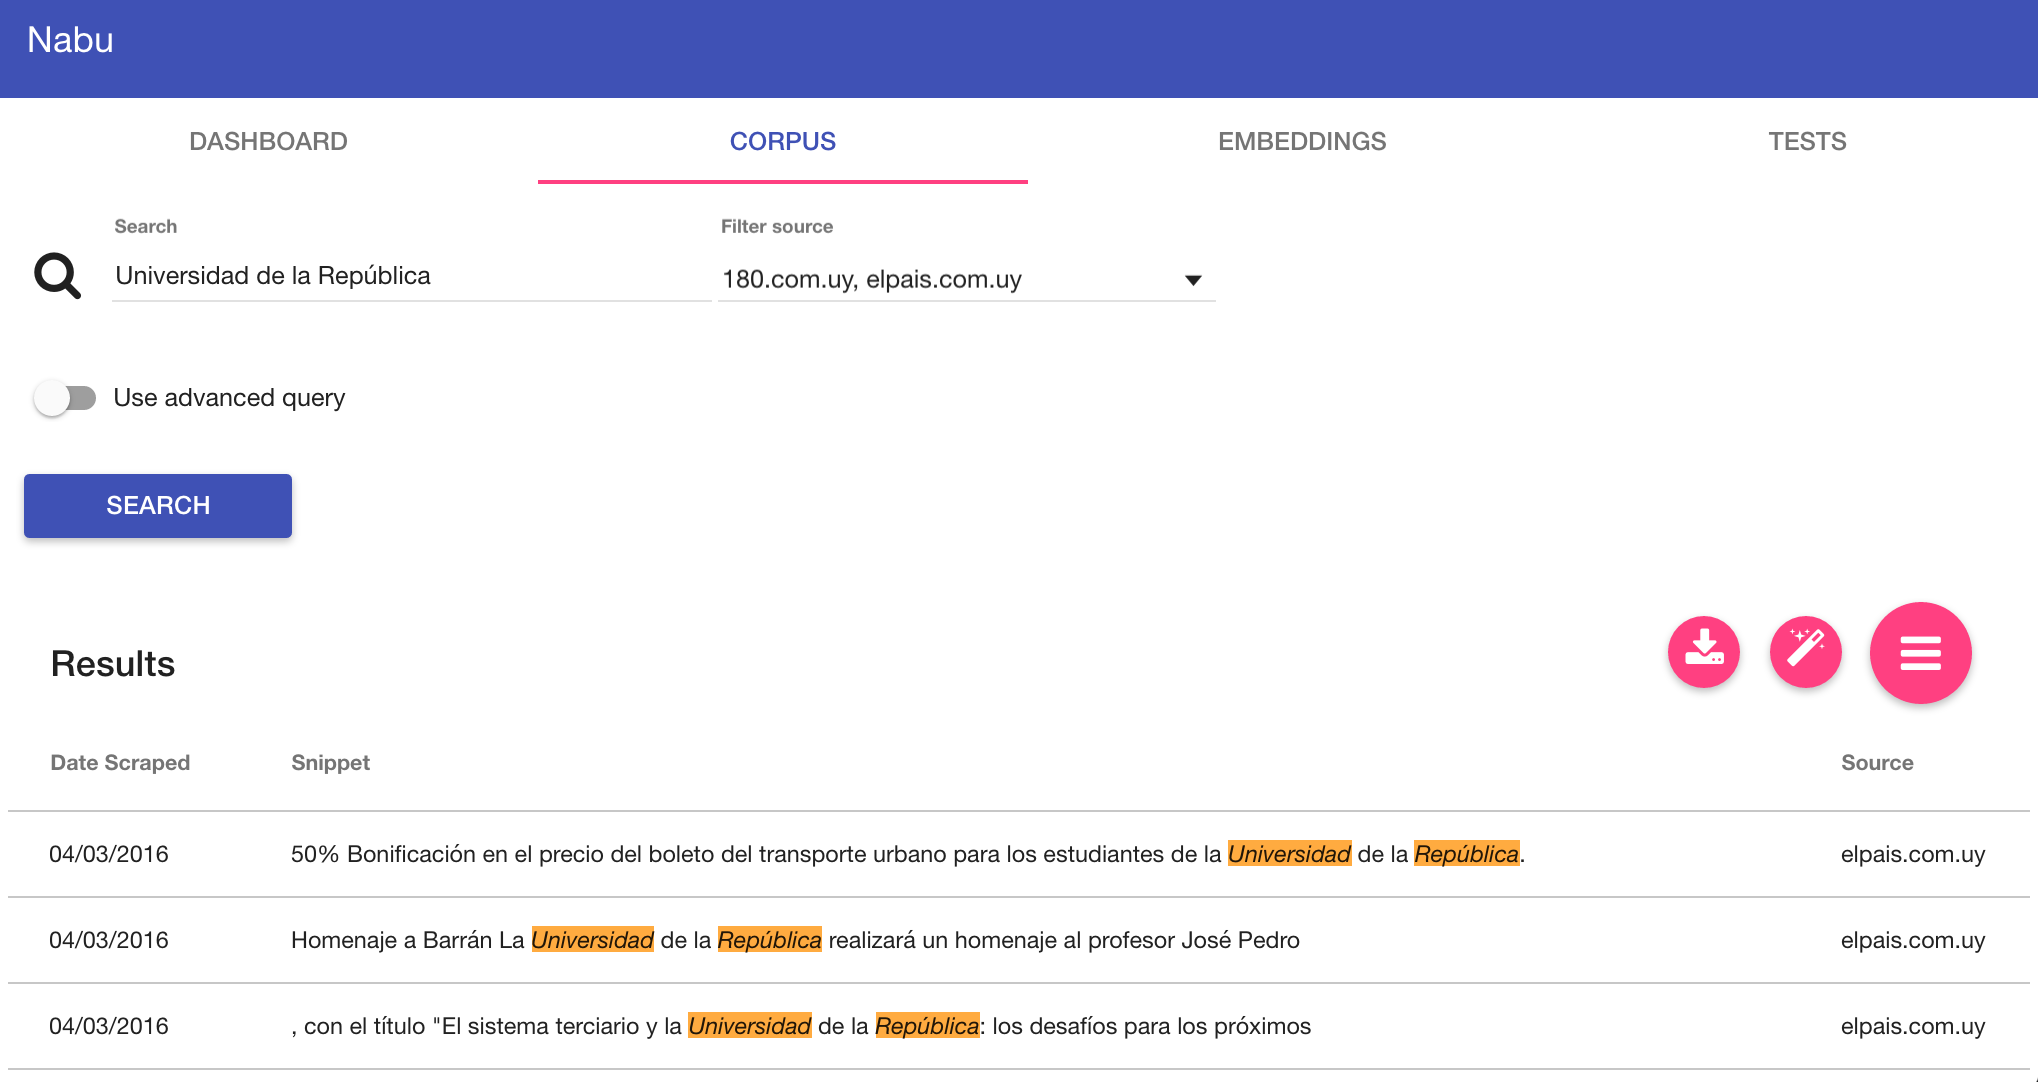
\includegraphics[width=\textwidth]{images/ui-nabu-corpus}
    \caption{\textit{Pantalla Corpus en la aplicación web.}}
    \label{fig:ui-nabu-corpus}
\end{figure}

Al hacer click en un documento de la tabla se presenta un cuadro de diálogo con información más detallada
del mismo. Se incluye cantidad de total de palabras, etiquetas, la fecha de creación en la fuente (si está
disponible) y el cuerpo completo del texto que lo compone. Se ofrece además un botón para abrir en una
nueva pestaña el documento en su fuente original, de modo de poder corroborar en cualquier momento la
fidelidad de los elementos del corpus.

En la vista principal se ofrecen además dos acciones adicionales. La primera de ellas permite descargar el
conjunto completo de documentos retornado al ejecutar la consulta, comprimidos en formato ZIP. La segunda
acción permite utilizar la consulta como entrada para crear una nueva representación vectorial, que se
entrenará con el subconjunto de documentos obtenido a partir de la consulta. Los detalles de creación de
vectores en el frontend se detallan más adelante. Pero dado que el corpus se encuentra en constante
crecimiento, es importante mencionar aquí que es recomendable especificar rangos de fechas de extracción en
las consultas al momento de crear nuevas representaciones vectoriales, de modo de permitir la posterior
reproducción de los resultados obtenidos.

\subsection{Embeddings}

En la sección \textit{Embeddings} se encapsulan la mayoría de las funcionalidades vinculadas a las
operaciones sobre representaciones vectoriales. En su vista principal se listan todas las representaciones
creadas en el sistema. De cada una se detalla su descripción, el tipo de modelo vectorial utilizado
(\texttt{word2vec}, \texttt{glove}, o \texttt{svd}), los parámetros de configuración del algoritmo elegido y
su estado de entrenamiento. Para cada vector los estados de entrenamiento posibles son \textit{entrenado},
\textit{en entrenamiento} y \textit{sin entrenar}.

\begin{figure}[h]
    \centering
    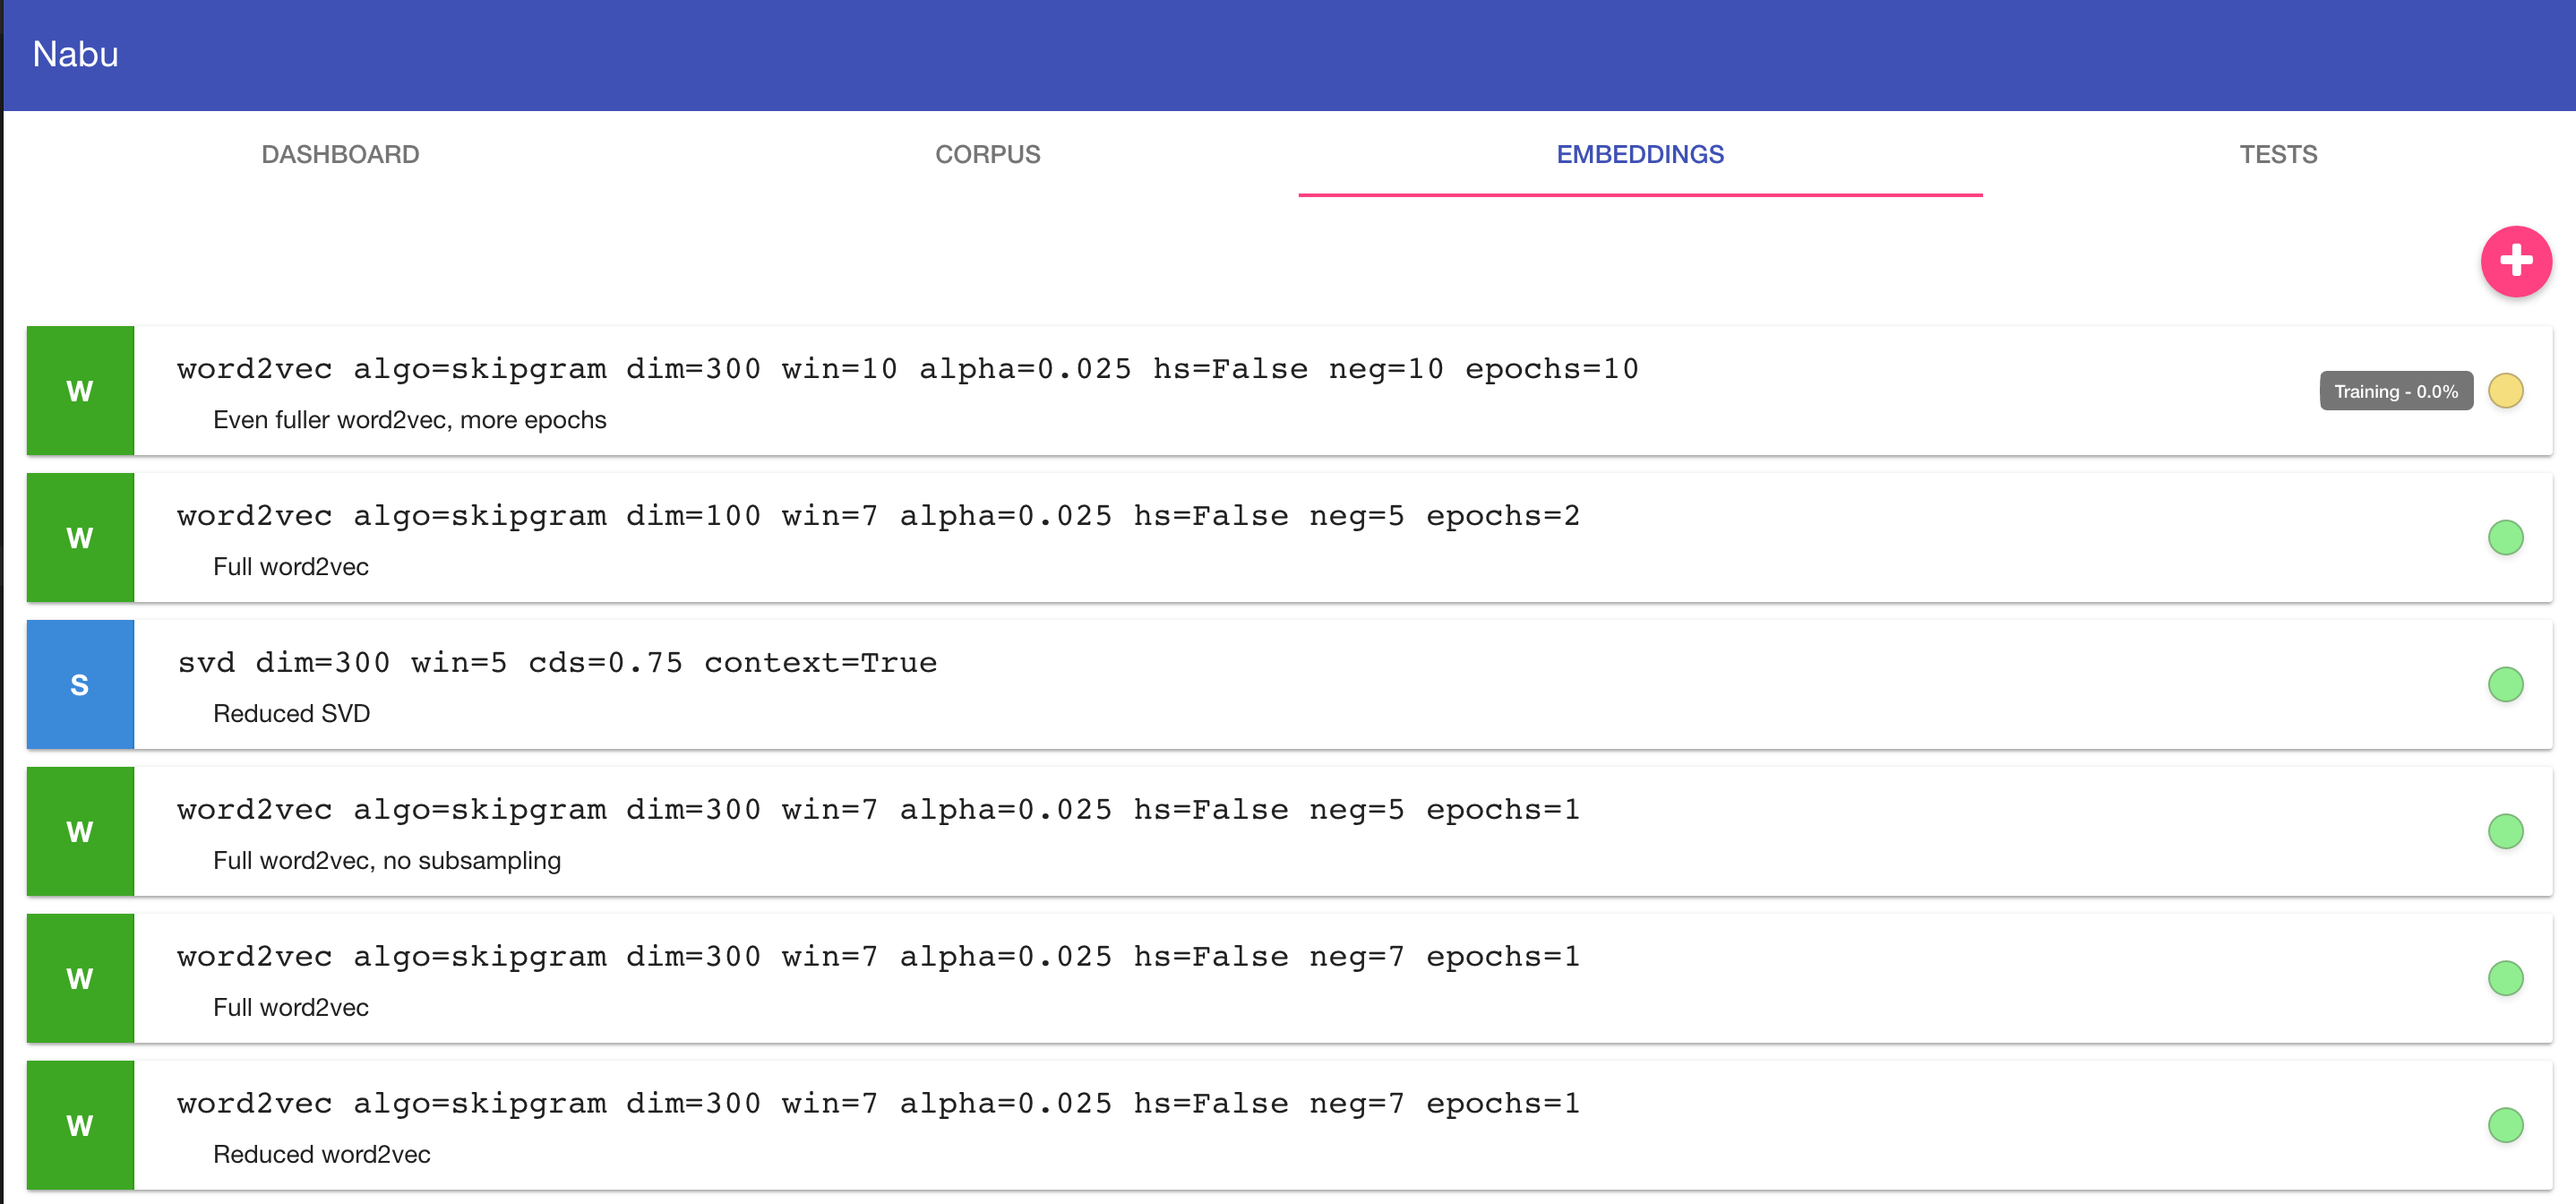
\includegraphics[width=\textwidth]{images/ui-nabu-embeddings}
    \caption{\textit{Pantalla Embeddings en la aplicación web.}}
    \label{fig:ui-nabu-embeddings}
\end{figure}

Esta vista ofrece un botón para crear y poner a entrenar una nueva representación vectorial. Al momento de
crear vectores se debe seleccionar uno de los tres modelos (en el caso de \texttt{word2vec} es necesario además
especificar el algoritmo a utilizar, \texttt{Skipgram} ó \texttt{CBOW}), fijar los valores de sus parámetros,
especificar la consulta en formato JSON que Elasticsearch utilizará para devolver los documentos de
entrenamiento y finalmente elegir los parámetros de preprocesamiento de texto. Una vez creada la representación
vectorial, esta será agregada a la cola de entrenamiento.

Al hacer click en las tarjetas de información de las representaciones vectoriales se accede a una vista en
detalle de las mismas. En los detalles, además de la información ya provista en la vista de listado, se incluye
el tamaño total en palabras del sub-corpus utilizado en el entrenamiento de la representación, el detalle
completo de los parámetros del modelo elegido, la consulta JSON utilizada para seleccionar los documentos de
entrenamiento y las opciones de preprocesamiento para el texto de dichos documentos. Cuando la representación
se encuentra en entrenamiento se incluye además una barra de progreso informando del avance actual en el
entrenamiento.

\begin{figure}[h]
    \centering
    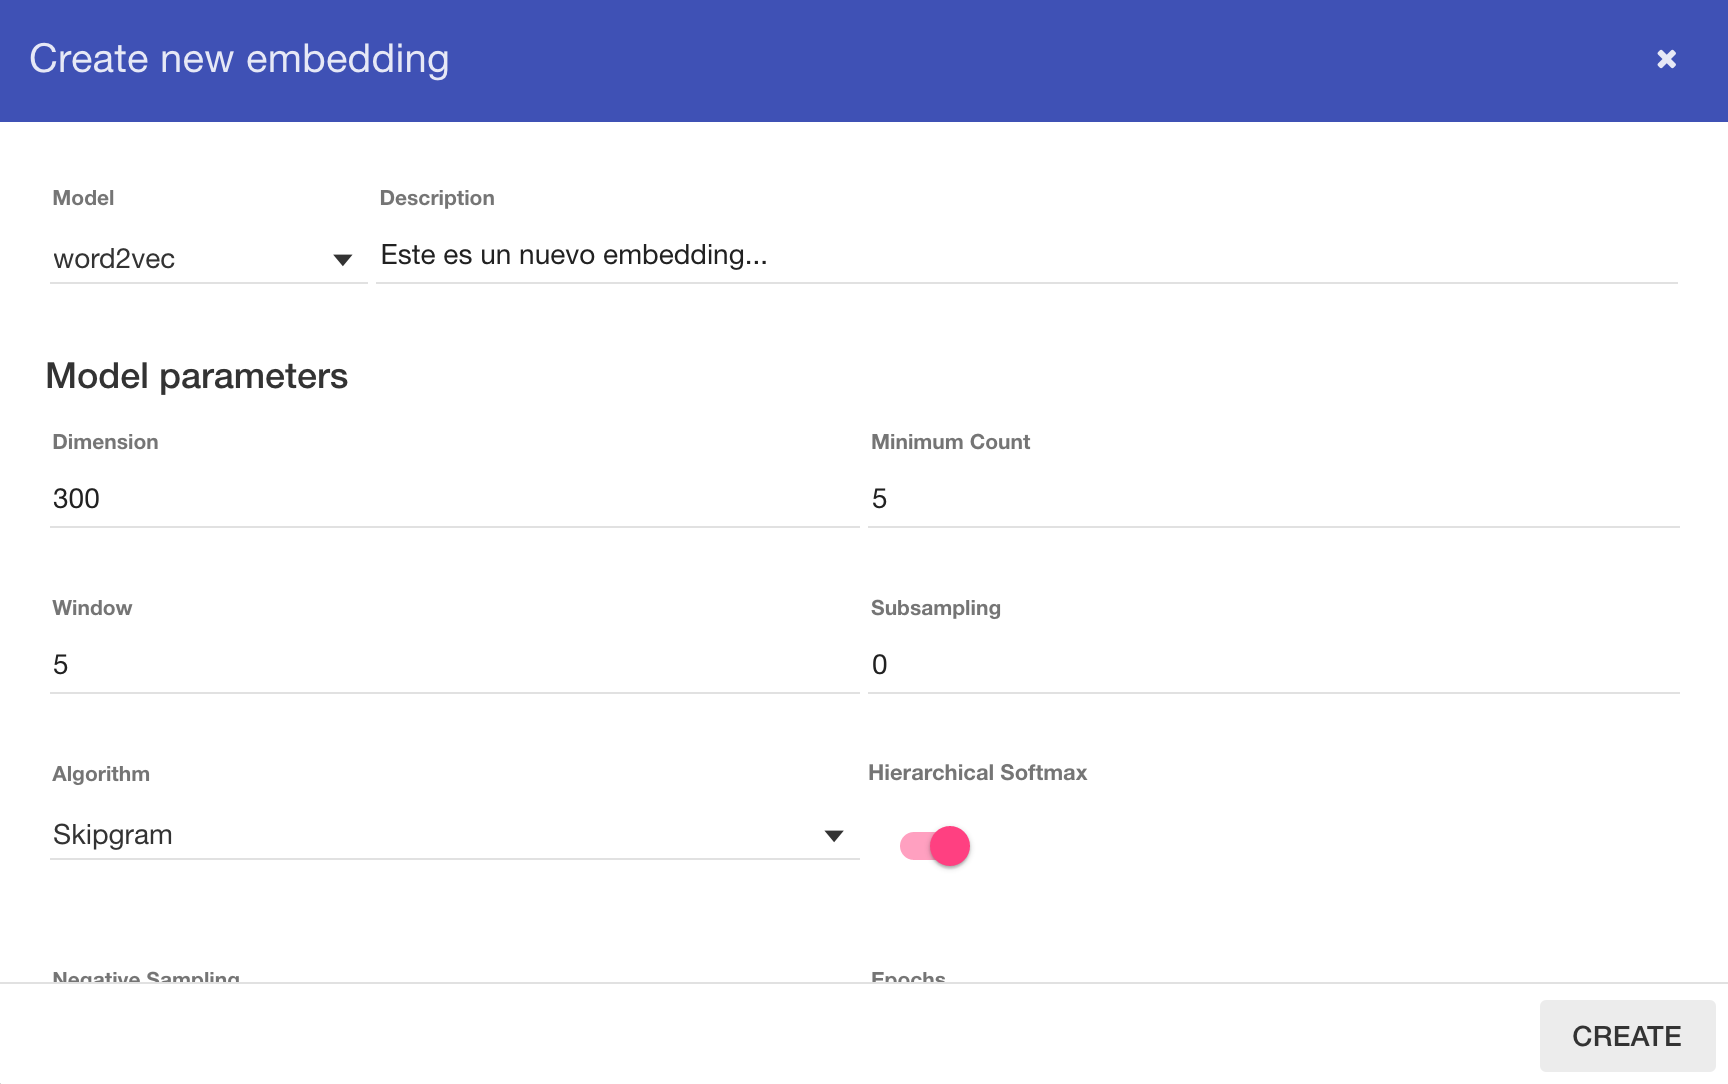
\includegraphics[width=\textwidth]{images/ui-nabu-embeddings-new}
    \caption{\textit{Pantalla para crear un nuevo Embedding en la aplicación web.}}
    \label{fig:ui-nabu-embeddings-new}
\end{figure}

De forma conveniente, junto al cuadro de la consulta en formato JSON se incluye un botón para ejecutar la
misma en la sección de \textit{Corpus}. Esto facilita la posibilidad de explorar el conjunto de documentos
utilizados para entrenar la representación vectorial. Eventualmente, un usuario podría descargar dicho conjunto
para entrenar una nueva representación de forma local utilizando el mismo algoritmo, de modo de verificar los
resultados logrados con la herramienta presentada en este proyecto.

Continuando con la descripción de la vista en detalle, se incluye al final de la misma una tabla con
información acerca de resultados de evaluación de la representación vectorial. En esta tabla se listan todos
los conjuntos de prueba con los que esta fue evaluada, la fecha de cada evaluación, el porcentaje de precisión
alcanzado en cada una y una botón para obtener una visión más detallada de los resultados de cada prueba.
Además, se incluye una columna que indica el desempeño de la representación en cada evaluación en comparación
con el resto de representaciones del sistema. Cuando la representación vectorial es la de mayor precisión en
una determinada prueba, se muestra un indicador del hecho junto a su posición.

La tabla de resultados de evaluación ofrece también una acción para ejecutar nuevas evaluaciones sobre las
representaciones vectoriales, permitiendo revaluar todas las pruebas, sólo evaluar aquellas aun no ejecutadas,
o evaluar un caso de prueba particular.

Finalmente se ofrecen acciones para eliminar la representación y para descargarla a la computadora del usuario.
La opción de descargar los vectores entrenados con la herramienta es una de las funcionalidad más valiosas e
importantes del proyecto. Esta funcionalidad permite a cualquier usuario interesado en el campo de las
representaciones vectoriales de palabras poder entrenar sus propias representaciones y luego descargarlas para
su uso en alguna aplicación de interés, sin la necesidad de poseer conocimientos detallados de los aspectos de
bajo nivel de las representaciones.

\subsection{Tests}

En la sección \textit{Tests} se encuentra toda la información relacionada a la evaluación de las
representaciones vectoriales de palabras creadas en el sistema. En su vista principal se presenta la lista de
casos de prueba disponibles, indicando para cada uno su nombre, descripción y categoría. Las categorías
principales son \textit{Analogías}, \textit{Similaridad} y \textit{Odd-one-out} (palabra que no encaja). De
forma conveniente, en esta vista se muestra también una pequeña medalla en cada caso de prueba con la cantidad
de representaciones que están siendo evaluadas actualmente, junto con un indicador de progreso de la tarea
actual.

\begin{figure}[h]
    \centering
    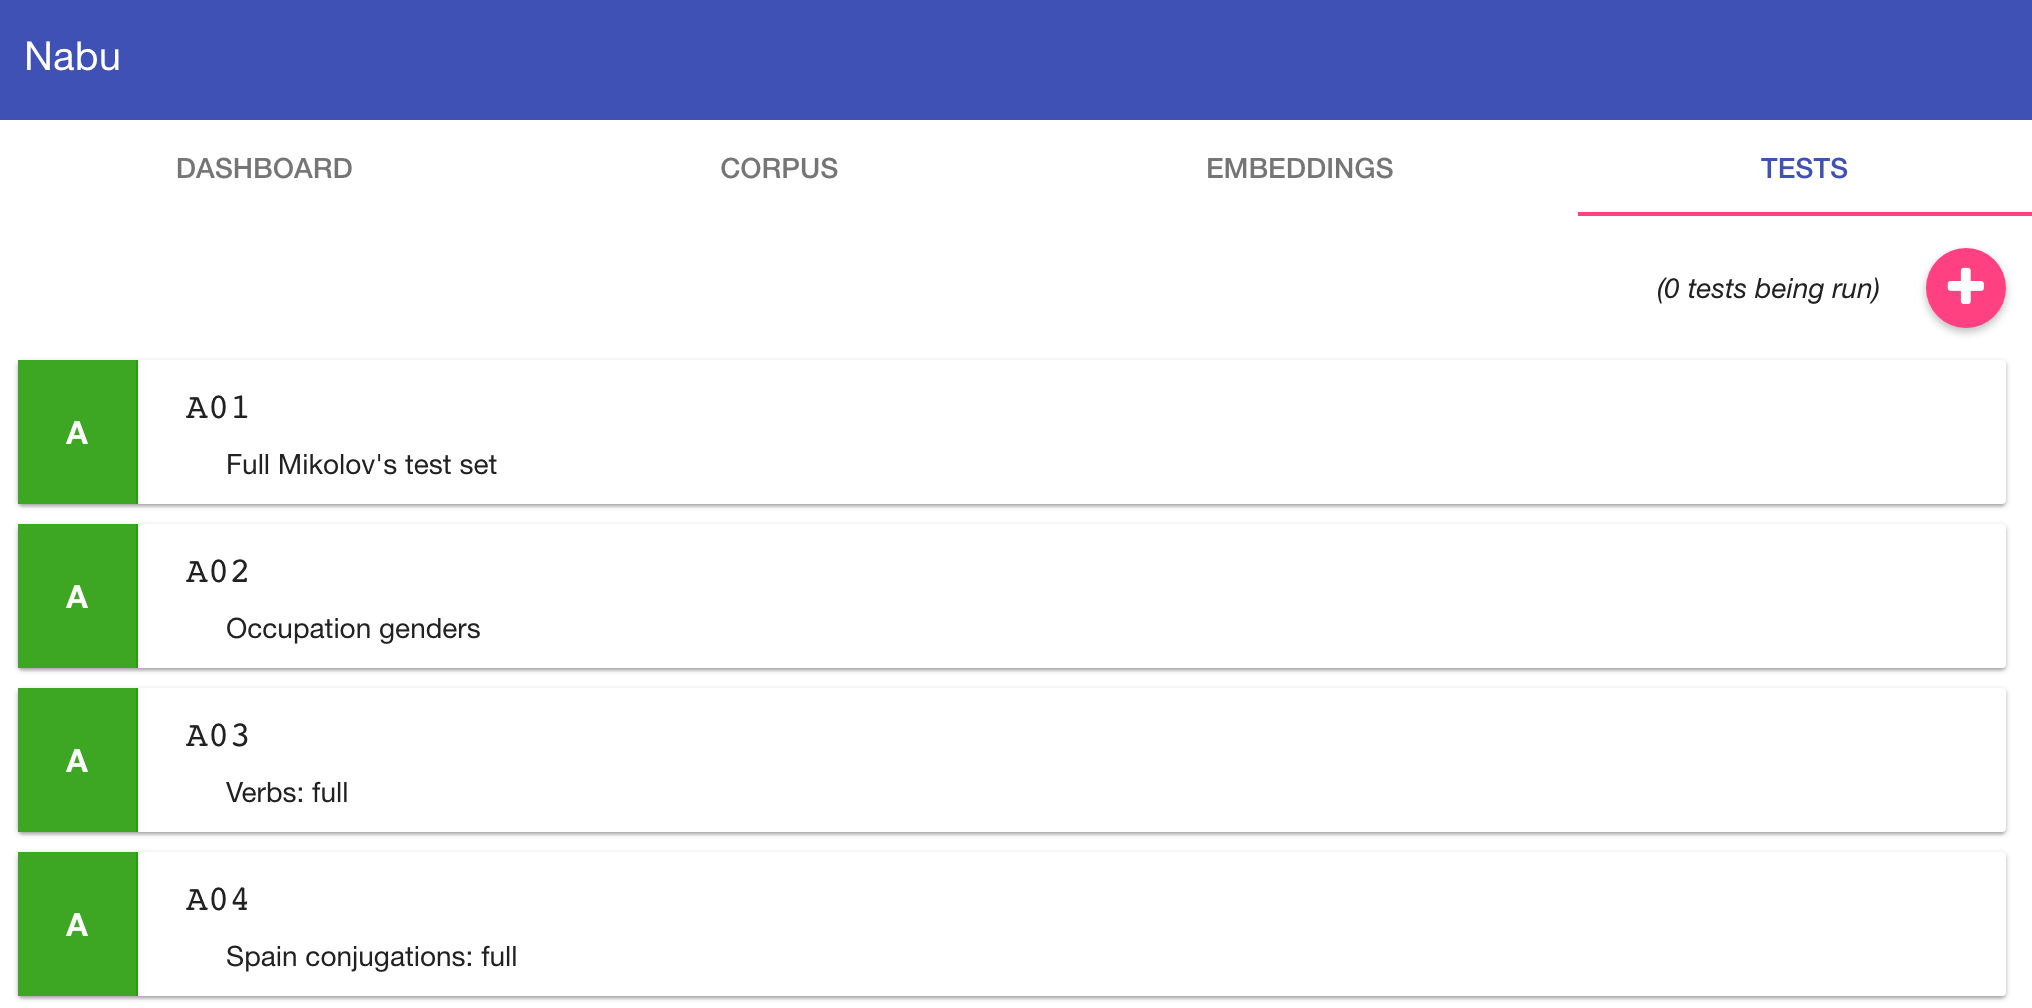
\includegraphics[width=\textwidth]{images/ui-nabu-tests}
    \caption{\textit{Pantalla Tests en la aplicación web.}}
    \label{fig:ui-nabu-tests}
\end{figure}

Los usuarios pueden hacer click en un caso de prueba para acceder a la vista de detalles, donde se
presenta información adicional. Además de los datos mostrados en la vista principal, se presenta un
ejemplo puntual del caso de prueba para mayor claridad de lo que se pretende evaluar. De manera adicional,
se muestran mayores detalles acerca de las tareas de evaluación que se están ejecutando en el momento.

En la vista de detalles se presenta también una tabla con resultados de evaluación. Para cada representación
evaluada con el caso de prueba se indica la fecha de la evaluación, un enlace a la página de detalles de la
representación, el modelo utilizado por la misma, el porcentaje de precisión logrado en el caso de prueba y
un botón para ver los detalles en profundidad de la evaluación. En los detalles en profundidad se
encuentra, cuando corresponde, el desempeño en las métricas \textsc{3CosAdd} y \textsc{3CosMul}
(porcentaje de aciertos exactos, y entre las primeras cinco y diez sugerencias), palabras no encontradas,
entradas faltantes, entradas equivocadas y cantidad total de entradas.

\begin{figure}[h]
    \centering
    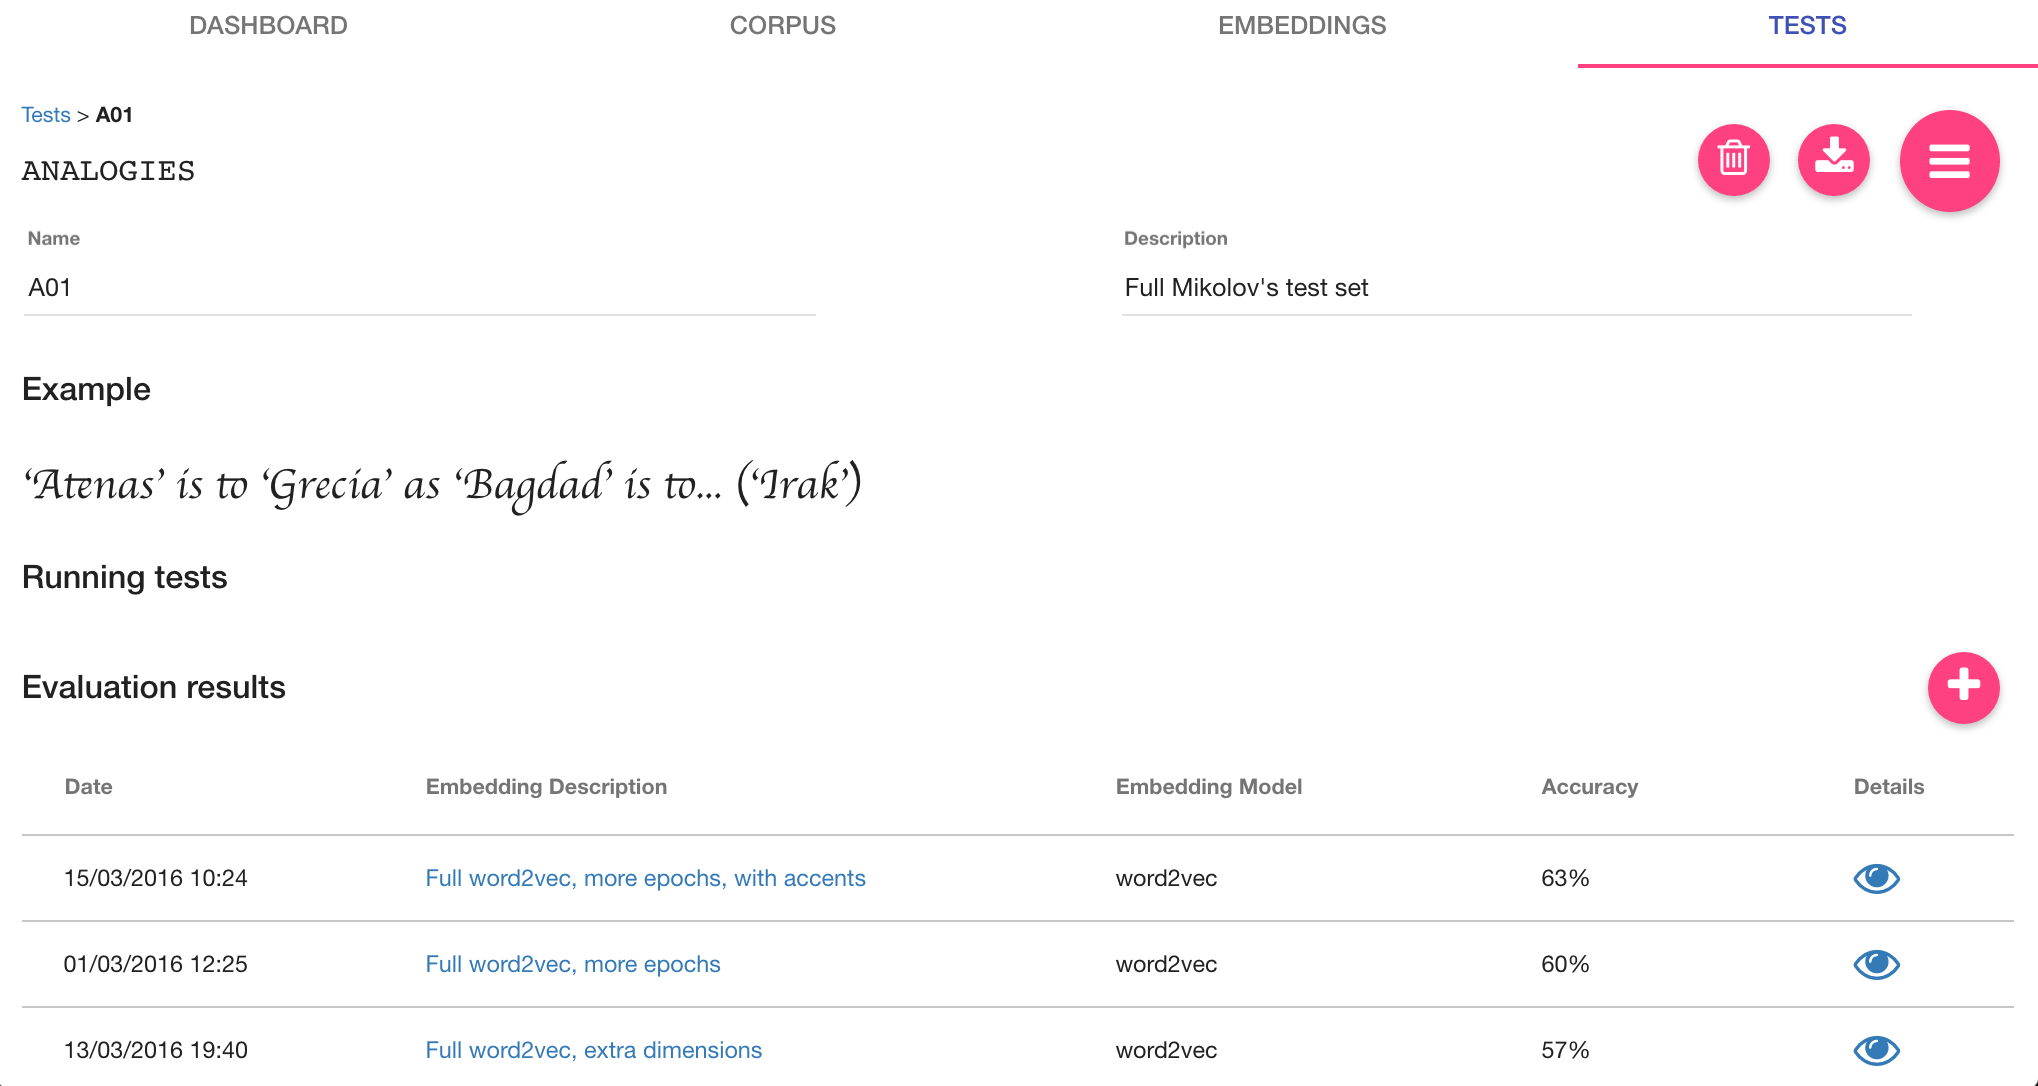
\includegraphics[width=\textwidth]{images/ui-nabu-tests-detail}
    \caption{\textit{Pantalla de vista en detalle de Tests en la aplicación web.}}
    \label{fig:ui-nabu-tests-detail}
\end{figure}

Desde la vista de detalles también es posible agendar nuevos trabajos de evaluación. Al momento de
crearlos se puede optar por elegir todas las representaciones que aun no fueron evaluadas con el caso de
prueba o por elegir uno en particular. También es posible optar por ejecutar el caso de prueba en todas las
representaciones vectoriales del sistema. En la parte superior de la pantalla se ofrecen además dos acciones
adicionales, una para eliminar el caso de prueba del sistema y otra para descargarlo en un archivo en formato
de cuatro columnas.

Finalmente, en la vista principal se cuenta con un botón que da acceso a un formulario para crear un
nuevo caso de pruebas en el sistema. En el formulario es necesario especificar nombre, descripción y
categoría para la nueva evaluación. Además es necesario subir un archivo de texto en formato de cuatro
columnas desde la computadora del cliente. Dicho archivo debe contener cuatro palabras separadas por un
espacio por línea, donde las primeras tres columnas se utilizarán en la evaluación y la cuarta es el
resultado esperado. El formato recién descrito es el mismo para las tres categorías existentes
actualmente, pero la semántica de cada columna depende de cada categoría, como bien se explicó en
secciones anteriores.


\section{Implementación}

En esta sección se presenta la implementación de la herramienta. Se comienza dando una descripción
de la arquitectura general de la misma, pasando luego a detallar la implementación de cada
módulo.


\subsection{Arquitectura General}

Dada la cantidad de requerimientos que se plantearon para la herramienta, fue necesario diagramar de
antemano una arquitectura que logre escalar y brindar todas las funcionalidades
satisfactoriamente. Ésta cuenta de seis componentes, o nodos, cada uno especializado en una función
distinta:

\begin{itemize}

\item Un nodo corriendo Elasticsearch, donde se almacena la totalidad del corpus de texto, como se
detalló en el capítulo anterior.

\item Un nodo corriendo PostgreSQL, donde se almacenan tanto las tablas relacionadas al scraping
automático como el modelo de datos empleado para la herramienta (esto es, información relacionada a
los modelos vectoriales entrenados y sus evaluaciones).

\item Un conjunto de nodos, denominados trabajadores o \textit{workers}, donde corren los algoritmos
para generar las representaciones vectoriales. Estos nodos son especiales en cuanto a que deben
contar con mayores recursos para poder entrenar los modelos en tiempos razonables. Su función es
consumir pedidos de una cola de tareas que indica qué algoritmo se debe entrenar a continuación, y
devolver el resultado.

\item Un nodo donde corre el servidor de aplicación que coordina los distintos componentes de la
arquitectura y ofrece una interfaz RESTful~\cite{Fielding2000} para interacción con el sistema. Sus
funciones incluyen la administración de la cola de tareas, la realización de consultas en Elasticsearch,
y la actualización del modelo de datos, entre otros.

\item Un nodo que sirve una aplicación web encargada de ofrecer una interfaz web sobre el servidor
de aplicaciones que pueda ser utilizada por un usuario no especializado.

\item Un nodo donde corre el proceso de scraping automático mencionado en el capítulo
anterior. Aunque no es técnicamente parte de la herramienta, se menciona por completitud.

\end{itemize}

Cabe notar que en la actualidad todos estos componentes corren en un único servidor con muchos
recursos (mencionado en el capítulo anterior), por no tener la herramienta demasiada demanda. Sin
embargo, es posible dividirlo en distintos servidores simplemente cambiando la configuración de los
nodos, permitiendo así escalar a un mayor número de usuarios de ser necesario.

La comunicación entre las distintas partes puede observarse en la figura~\ref{fig:diag-tool-arch}.
En el centro de la arquitectura se encuentra el servidor de aplicación, que se encarga de coordinar
el resto de los nodos. Éste ofrece una API (o \textit{Application Programming Interface}) RESTful
que permite realizar consultas sobre el corpus, crear nuevos modelos vectoriales, enviarlos a entrenar
y evaluar, y todo el resto de las funcionalidades que ofrece la herramienta. Tiene, por lo tanto, que
comunicarse con el nodo de Elasticsearch, con el nodo de PostgreSQL, y mantener la cola de tareas
que los \textit{workers} posteriormente consumirán.

Los nodos workers también deben comunicarse con Elasticsearch, para obtener el contenido del
corpus de entrenamiento, y con PostgreSQL, para actualizar el estado de los modelos vectoriales que
se entrenan o evalúan.

Por otro lado, la aplicación web se comunica únicamente con el servidor de aplicaciones, pues la
interfaz de este último es capaz de abstraer toda la maquinaria interna de la herramienta. Por esta
razón, denominamos la aplicación web como la parte delantera de la aplicación (o \textit{frontend})
y al resto de los nodos (el servidor de aplicación y los otros nodos) la parte trasera (o
\textit{backend}).

\begin{figure}[h]
    \centering
    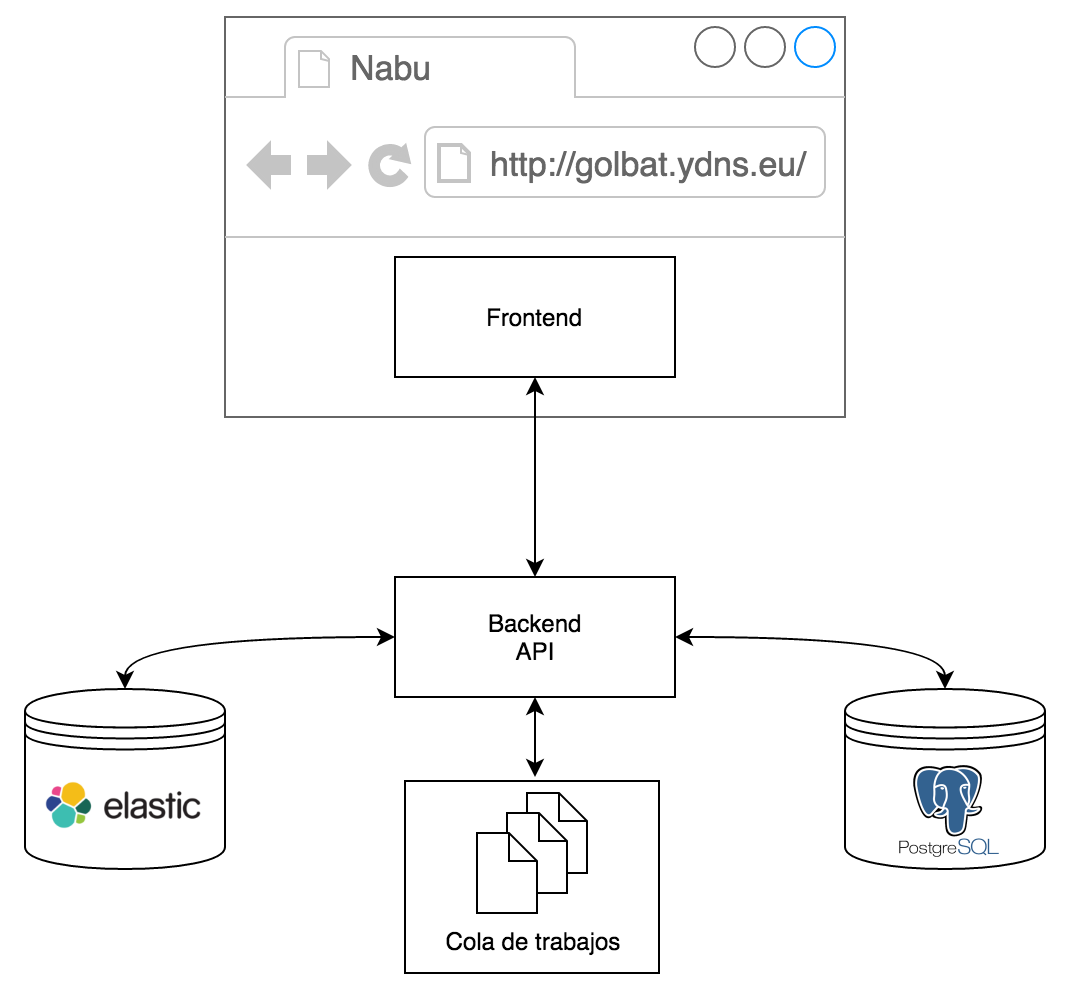
\includegraphics[width=\textwidth]{images/diag-tool-arch}
    \caption{\textit{Arquitectura a alto nivel de la herramienta.}}
    \label{fig:diag-tool-arch}
\end{figure}


\subsection{Backend}

El \textit{backend} de la aplicación busca, como se mencionó anteriormente, brindar una interfaz
RESTful capaz de abstraer las particularidades de la implementación de la herramienta. Internamente
se encarga de la comunicación con Elasticsearch (donde se almacena el corpus) y PostgreSQL (donde se
mantiene el estado de la aplicación), y de coordinar y realizar el entrenamiento y evaluación de los
vectores de manera distribuida a través de una cola de tareas. Permite también la interacción con
los datos que componen el estado de la aplicación.


\subsubsection{Modelo de Datos}

Empezaremos detallando el modelo de datos que define al dominio con el que trata la herramienta:

\begin{itemize}

\item En primer lugar, se cuenta con modelos (esto es, tablas en la base de datos) para las
representaciones vectoriales que se registraron en la herramienta. Para cada una de ellas se guarda
el algoritmo empleado para su generación, los hiperparámetros del mismo (que dependen, claro está,
del algoritmo), la consulta de Elasticsearch a través de la cual se obtiene el corpus de
entrenamiento, y el tipo de preprocesamiento empleado para tratar el texto previo a entrenar.

Además almacena la fecha de creación y el estado actual del modelo, que puede ser \textit{sin
entrenar}, \textit{entrenando}, o \textit{entrenado}, dependiendo si ya se corrió el algoritmo o
no. En caso de que ya se haya entrenado, se guarda también una referencia a la ubicación de los
archivos de los vectores.

\item También se cuenta con modelos para los distintos conjuntos de prueba dados de alta en el
sistema. Para cada uno de ellos se registra el tipo de pruebas (esto es, si son analogías, similitud
de palabras, etc.) y la ubicación del archivo que contiene los datos de prueba. Por comodidad,
también se les puede asignar un nombre y una descripción.

\item Se emplean modelos adicionales para almacenar los resultados de las evaluaciones de los
distintos vectores de palabras. Cada uno de estos cuenta con referencias al modelo vectorial y el
conjunto de pruebas a los que describe, junto con los resultados obtenidos en la evaluación (esto
es, la precisión y otros datos, dependiendo del tipo de prueba).

\item Por último, se cuenta con modelos para registrar las tareas (o \textit{jobs}) que corren en
los nodos trabajadores para el entrenamiento y evaluación de los vectores. Su funcionamiento se
describirá más adelante, pero se puede mencionar que se guardan datos acerca del tiempo empleado y
fecha de agendado de la tarea, para poder luego estudiar el tiempo de cómputo requerido para generar
las representaciones.

\end{itemize}


\subsubsection{Cola de Tareas}

Para el entrenamiento de vectores, se ideó una arquitectura basada en una cola de tareas (o
\textit{job queue}) en el que el servidor de aplicación da de alta tareas que serán luego llevadas a
cabo por nodos trabajadores (o \textit{workers}), los cuales cuentan con amplios recursos
computacionales para correr los algoritmos. Esto es necesario ya que los algoritmos pueden demorar
horas e incluso días en finalizar, por lo que es imposible correrlos en el tiempo en que se debe
atender un pedido HTTP\@.

Se utilizó la biblioteca Celery~\cite{Celery} para la comunicación y la administración de dicha
cola. Celery ofrece un mecanismo para producir y consumir mensajes en una cola de tareas en tiempo
real, a través de un sistema distribuido, flexible, y confiable, lo que lo hace una buena opción
para la herramienta a construir. A través de esta biblioteca, es posible definir tipos de tareas
(como puede ser entrenar o evaluar un modelo vectorial) y luego dar de alta mensajes que serán
consumido por nodos trabajadores, los cuales se encargarán de correr el código necesario y devolver
el resultado.

Celery se limita a coordinar el uso de la cola de tareas, por lo que toda la información adicional
que sea necesaria almacenar respecto a las tareas (identificadores y resultados, por ejemplo), debe
ser mantenida por una base de datos especializada. Para la presente arquitectura se decidió utilizar
Redis, un almacén de estructuras de datos en memoria, por ser una solución simple y liviana.

Se definen dos tipos de tareas que el sistema correrá de manera asincrónica: una para el
entrenamiento de representaciones vectoriales y otra para la evaluación de las mismas. El primer tipo
recibe el modelo vectorial a entrenar (esto es, el algoritmo a utilizar, sus hiperparámetros, la
consulta de Elasticsearch que describe al corpus de texto, y las opciones de preprocesamiento de los
datos) y luego procede a correr el algoritmo, reportando el progreso periódicamente. Una vez
finalizado, actualiza los registros asociados a los vectores en la base de datos (pasando el estado
de la tarea a \textit{entrenado}, por ejemplo) y los persiste en el sistema de archivos del
servidor.

El segundo tipo de tarea recibe el modelo vectorial (ya entrenado) a evaluar y el conjunto de
pruebas a utilizar. Una vez cargados todos los datos en memoria, procede a realizar la evaluación,
la cual dependerá del tipo de prueba que se está realizando (esto es, si es una tarea de analogías o
de similitud de palabra, por ejemplo). Reporta el progreso conforme avanza con la evaluación y
finalmente almacena el resultado en la base de datos. En caso de ya existir un resultado para la
combinación de vectores y pruebas, lo sobreescribe.

Para cada tipo de tarea, es necesario mantener ciertos metadatos asociados a la misma, por lo que se
mantiene una tabla para cada una con este fin, como se mencionó anteriormente. En éstas se almacena
información pertinente para la ejecución de la tarea (modelos vectoriales y conjuntos de pruebas
sobre los que actuar, principalmente) e información sobre la tarea en sí. En particular, se registra
un identificador (denominado \texttt{task\_id}) con el que se puede consultar el progreso y el
estado de la tarea a través de Celery. También se almacenan otros metadatos como la fecha de
agendado y el tiempo de ejecución de la tarea.

Al recibir un pedido a través de la API para entrenar un modelo vectorial particular, el servidor de
aplicación da de alta una nueva tarea en la cola mediante Celery, creando también un registro
asociado en la base de datos, y devolviendo al pedido HTTP el identificador de la tarea. Por detrás,
un nodo trabajador recibirá la tarea a ejecutar y la iniciará, cambiando el estado de la misma a
\textit{entrenando} y reportando el progreso periódicamente. Mientras ejecuta, el usuario puede
realizar otro llamado a la API para consultar el estado de la tarea utilizando el identificador de
la misma. Una vez finalizada la ejecución el estado pasará a \textit{entrenado} y, cuando el
usuario vuelva a consultar por el progreso, se le indicará que ya ha terminado. Esto lo habilitará a
descargar o evaluar el modelo.

Para la evaluación de modelos el procedimiento es análogo, con la diferencia que a través de un
único llamado a la API es posible evaluar un modelo en varios conjuntos de prueba o vice versa.
Para ambos casos (entrenamiento y evaluación) se tienen consideraciones especiales cuando se crea
una tarea si la misma está actualmente en ejecución o ya ha terminado: para el entrenamiento de un
vector, se devolverá un error, mientras que para la evaluación se borrarán primero los resultados
existentes.

En la figura~\ref{fig:diag-tool-flow} se diagrama el funcionamiento del procedimiento completo. Se
muestra además cómo interactúan los distintos componentes de la cola de tareas entre sí y cómo se
comunican con el resto de los nodos del sistema.

\begin{figure}[h]
    \centering
    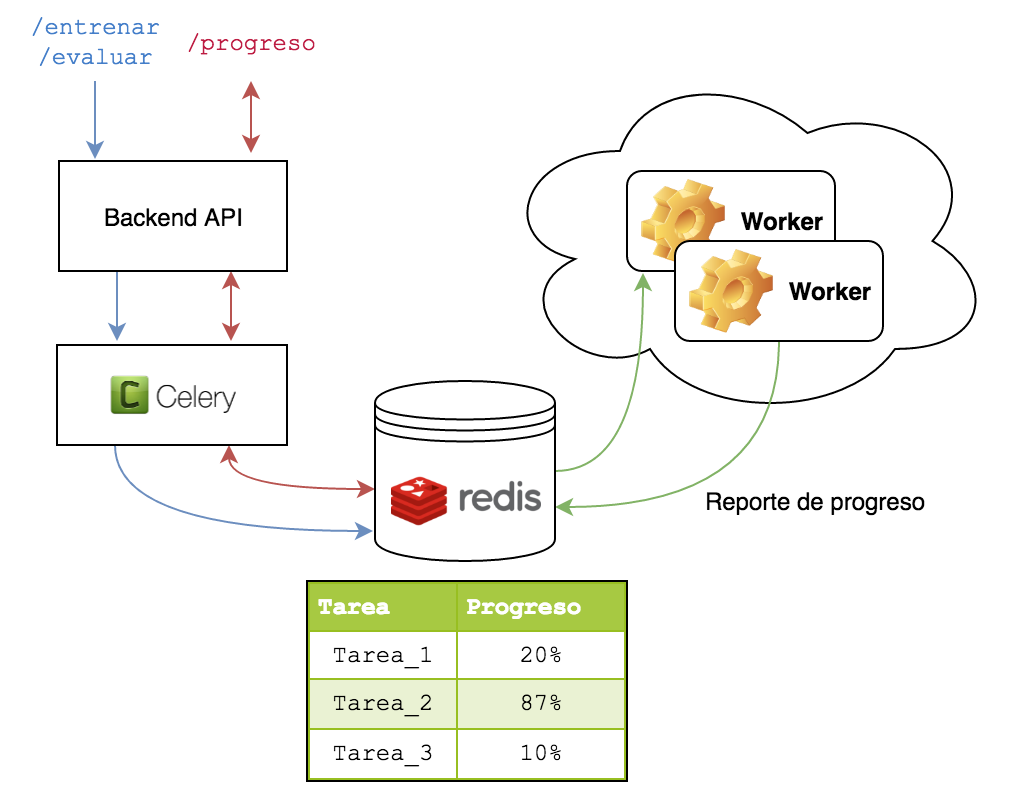
\includegraphics[width=\textwidth]{images/diag-tool-flow}
    \caption{\textit{Diagrama del proceso empleado para el entrenamiento y la evaluación de vectores.}}
    \label{fig:diag-tool-flow}
\end{figure}


\subsubsection{Entrenamiento}

Con el fin de evitar errores de implementación en los algoritmos para generar representaciones
vectoriales, se buscó, donde fue posible, aprovechar bibliotecas ya existentes y probadas.

\paragraph{word2vec}

Debido a su popularidad, existen varias implementaciones de \texttt{word2vec} en la comunidad. En
primer lugar se encuentra, claro está, la implementación de los algoritmos CBOW y SGNS hechas por
Mikolov~\cite{Word2vecGoogle}. También existen implementaciones en diversos lenguajes de programación,
como la provista por \texttt{Gensim} (escrita en Python~\cite{RehurekLrec}), o la provista por
\texttt{mllib} (escrita en Java~\cite{Word2vecMLlib}), entre otras.

Se optó por utilizar la implementación de la biblioteca \texttt{Gensim} pues el hecho de estar
escrita en Python facilita mucho su integración con el resto del sistema. Además, como muestran los
contactos que tuvo el autor de la misma con Mikolov~\cite{MikolovGoogleGroups}, es una implementación
probada que llega incluso a ser más eficiente computacionalmente que la original, a pesar de estar
escrita en Python.


\paragraph{GloVe}

Para el caso de GloVe se decidió utilizar la implementación provista por los autores~\cite{Pennington2014},
pues no existen bibliotecas satisfactorias escritas en Python. Por esta razón la tarea de integración fue
más compleja, pues fue necesario utilizar el módulo Python \texttt{subprocess} para comunicarse con
un proceso hijo que corre los algoritmos, trasmitiendo el texto del corpus a través de la entrada
estándar del mismo.


\paragraph{Modelo Estadístico}

Para el cuarto algoritmo, el modelo estadístico basado en la matriz PPMI con SVD, fue necesario
realizar una implementación propia, pues no fue posible encontrar ninguna que cumpliera con los
requerimientos necesarios. Partiendo del artículo de Levy y Goldberg~\cite{Levy2015}, y aprovechando
parte del código provisto por los autores en ~\cite{LevyHyperwords}, se elaboró un módulo Python para
la construcción de representaciones con dicho modelo.

Se utilizaron las bibliotecas \texttt{numpy}~\cite{NumPy} y \texttt{scipy}~\cite{SciPy} para la
manipulación numérica de matrices (matrices dispersas, en particular, como lo es la matriz de coocurrencias
con medida PPMI), y el \textit{wrapper} \texttt{sparsesvd}~\cite{sparsesvd} de la biblioteca
\texttt{SVDLIBC}~\cite{SVDLIBC} para la aplicación de SVD a matrices dispersas.

Teniendo en cuenta algunas sugerencias de los autores en cuanto al tratamiento efectivo de matrices
dispersas (en lo que respecta al uso de memoria principalmente), se logró a una implementación
satisfactoria del algoritmo con un comportamiento similar al que describen los autores en el
artículo original. Se implementan también las heurísticas que los autores encuentran que favorecen
la performance del algoritmo, como el \textit{subsampling} de palabras comunes y la eliminación de
palabras poco frecuentes.


\subsubsection{Evaluación}

Se implementaron tres mecanismos de evaluación para las representaciones vectoriales, a
continuación se describe el proceso de implementación para cada uno.


\paragraph{Analogías}

El primero de ellos es la tarea de analogías, descrita anteriormente, donde se debe obtener una
palabra ($w_4$) en base a otras tres ($w_1$, $w_2$, $w_3$) bajo el esquema ``$w_1$ es a $w_2$ lo que
$w_3$ es a $w_4$''.

Los conjuntos de pruebas para esta tarea se componen de una lista de 4-uplas con las palabras que
forman la analogía, donde la última es que se debe recuperar. El \textit{job} encargado de correr la
evaluación leerá el archivo con los datos (una analogía por línea) y utilizará las métricas
\textsc{3CosAdd} y \textsc{3CosMul} para obtener el resultado, como se especifica en el capítulo
2.

Se almacena el porcentaje de aciertos exactos, el porcentaje de aciertos entre las cinco primeras
sugerencias, y el porcentaje de aciertos entre las diez primeras sugerencias. De esta forma se puede
estimar, en caso de que haya fallado la recuperación, qué tan cerca se estuvo. Se registra también
la cantidad de palabras que no se encontraron en el vocabulario del modelo para tener una idea de
qué tanto afecta esto al resultado final, pues la ausencia en el vocabulario cuenta como un
fallo\footnote{Si no contara como un fallo, un modelo vectorial con un vocabulario de diez palabras
podría tener un porcentaje de aciertos perfecto en todas las pruebas.}.


\paragraph{Similitud}

El segundo mecanismo de evaluación es la similitud de palabras. Esta tarea asigna un puntaje entre 0
y 10 a la similitud o relación entre pares de palabras, donde 10 significa que una palabra puede ser
sustituida por otra en un contexto dado (caso similitud) o son palabras que están estrechamente
relacionadas (caso relación).

La prueba en sí consiste en cargar la lista de pares de palabras, asignar un puntaje a cada par de
palabras (utilizando la distancia coseno entre sus representaciones vectoriales) y calcular la
correlación entre los puntajes obtenidos y los del conjunto de pruebas (que son asignados por jueces
humanos). Esta es la técnica estándar en la literatura para evaluar la capacidad de capturar
relaciones de similitud por parte de los vectores de palabras, como se vio en el capítulo 2.

Los archivos con los datos de prueba consisten en una lista de dos palabras y su puntaje de
similitud asociado. Por otro lado, y al igual que en las analogías, se guarda también la cantidad de
palabras que no se encontraron en el vocabulario.


\paragraph{Odd-one-out}

El tercer mecanismo de evaluación consiste en encontrar la palabra que no encaja en un conjunto de
palabras (encontrar el \textit{odd-one-out}). Por ejemplo, la palabra \textit{auto} en el conjunto
de palabras \textit{auto}, \textit{rótula}, \textit{pelvis}, y \textit{metatarso}. Se pueden
construir, por ejemplo, pruebas tanto por campo semántico (como el recién ejemplificado) como por
campo sintáctico (donde se busca, por ejemplo, identificar al verbo con conjugación distinta).

No existe mucho trabajo en la literatura con este esquema de pruebas, pero aun así es útil para
comparar los distintos tipos de representaciones entre sí, en una tarea que busca medir también qué
tanto se capturan las similitudes entre palabras.

El conjunto de pruebas consta de una lista de palabras (de largo variable) donde la primera es la
palabra que no encaja. Para obtener cuál es dicha palabra, se toma el centroide (el promedio
componente a componente de los vectores) y se devuelve la palabra más lejana al mismo. En este caso
se almacenan la cantidad de resultados donde ninguna palabra está presente en el vocabulario; se
considera aceptable que falten palabras mientras que sea capaz de obtener correctamente el
resultado.

\quad

Cabe notar también que al momento de evaluar los modelos vectoriales se le aplica a las palabras del
conjunto de pruebas el mismo preprocesamiento que se le aplicó al corpus de texto al construir los
vectores. Así se evitan problemas de incompatibilidad entre las pruebas y las representaciones
(donde uno saca los tildes y el otro no, por ejemplo).


\subsubsection{API HTTP}

El último gran componente del backend es la API web, cuyo objetivo es brindar una interfaz HTTP
RESTful que permita interactuar con toda esta maquinaria ya descrita, buscando en lo posible
esconder las complejidades de la misma. Esto es, se busca que el usuario que utilice esta API no
requiera conocimiento de Celery, ni de PostgreSQL, ni de la implementación particular de los
algoritmos y evaluaciones utilizados, ni de ningún otro componente interno del sistema. Así, para el
usuario, los modelos vectoriales estarán siendo entrenados por una caja negra que devuelve una lista
de vectores con determinadas características al finalizar.

Con este fin, la API se maneja exclusivamente a nivel del modelo de datos: esto es, el usuario
interactúa con recursos REST~\cite{Fielding2000} que representan al dominio del sistema que se
describió antes, junto con un recurso especial para la búsqueda de documentos en el corpus.

El principal objetivo de esta interfaz es ser consumida por el frontend de la herramienta, aunque
puede ser utilizada por un usuario realizando los pedidos HTTP manualmente si así lo desea.


\paragraph{Corpus}

Se exponen tres \textit{endpoints} (URLs que referencian a un recurso particular) relacionados con
el corpus de texto, todos bajo el prefijo \texttt{/corpus/}. El primero de ellos,
\texttt{/corpus/search/} permite realizar una búsqueda en el texto, filtrando por la aparición de
uno o más términos determinados o por campos de los metadatos asociados a cada documento. La
consulta se especifica a través de un documento JSON~\cite{JSON}, siguiendo el formato empleado por
Elasticsearch, por lo que ofrece toda las funcionalidades que este motor de búsqueda brinda. Para
cada documento recuperado, se devuelve fragmento de su contenido, con el texto que coincide con el
término de búsqueda resaltado. También se provee funcionalidades de paginado para no tener problemas
con consultas demasiado grandes.

A través del endpoint \texttt{/corpus/document/<id>/}, es posible recuperar un documento en su
totalidad, con el contenido completo y todos sus metadatos. En caso de existir, también se provee
una URL para acceder al documento directamente en la fuente correspondiente.

Puesto que recorrer todo el corpus documento a documento a través de los anteriores llamados sería
extremadamente ineficiente, se provee un endpoint adicional, \texttt{/corpus/download/}, que, a
partir de una consulta con el mismo formato de las búsquedas, devuelve un archivo con el contenido
de todos los documentos que coinciden con la misma. Para ello, se recuperan los documentos y se
construye un archivo comprimido en formato ZIP~\cite{ZIPFormat} compuesto por un archivo de texto
plano por documento.

Dado que los contenidos asociados al resultado de una consulta podrían ocupar un gran tamaño (en el
orden de \textit{gigabytes}), es imprescindible este archivo no se genere por completo en el
servidor y que luego se envíe al usuario. Con este fin, se utilizó la biblioteca de Python
\texttt{zipstream}~\cite{zipstream}, que permite ir construyendo y sirviendo el contenido de un archivo
ZIP mientras el usuario lo va descargando, agregándole los archivos con el contenido de los documentos
uno a uno, logrando así que el archivo final nunca se almacene por completo en el servidor.

Por otro lado, cabe notar que permitir al usuario ingresar una consulta genérica a través de la API
plantea ciertas consideraciones de seguridad. Dado que la entrada del usuario se restringe a una
consulta sobre el corpus, no podrá modificar el contenido almacenado. Sin embargo, fue necesario
tomar precauciones adicionales y bloquear la funcionalidad de consultas con scripts de Elasticsearch
~\cite{ElasticsearchScripting} para evitar inconvenientes\footnote{De hecho, las nuevas versiones de
Elasticsearch vienen con esta funcionalidad deshabilitadas por este mismo motivo.}.


\paragraph{Vectores y Pruebas}

La API también brinda funcionalidades para manipular vectores de palabras, conjuntos de pruebas y
resultados. Para cada uno de estos tres recursos, es posible crearlos, obtener sus detalles (a
través de un identificador asignado a cada uno, e.g. \texttt{/embeddings/1/}), listarlos,
modificarlos, y eliminarlos.

En el caso de las representaciones vectoriales, la vista detallada devuelve qué algoritmo se utilizó
para entrenar, los hiperparámetros empleados, el corpus utilizado (la consulta de Elasticsearch, el
tamaño en cantidad de palabras, y las opciones de preprocesamiento), y si ya ha sido entrenado o
no. Es posible asignarles una descripción para poder identificarlos más fácilmente. También es
posible descargar los vectores a través del endpoint \texttt{/embeddings/<id>/download/}, donde se
emplea una técnica similar a la descrita en la sección anterior para devolverle al usuario los
archivos asociados a dicho modelo.

Los conjuntos de pruebas devuelven el tipo de prueba que contienen (e.g.\ analogías), junto con un
nombre y una descripción asignadas por el usuario. Se devuelve también un ejemplo de la prueba, para
que el usuario tenga como referencia (por ejemplo, ``\,`increíble' is to `increíblemente' as
`aparente' is to\ldots (`aparentemente')''). Al igual que en los vectores, es posible descargar los
datos del conjunto de pruebas a través del endpoint \texttt{/testsets/<id>/download/}, donde se
devuelve directamente un archivo de texto plano con las entradas.

Para los dos anteriores casos, sólo es posible modificar el nombre y descripción de los recursos; en
caso de querer cambiar, por ejemplo, los hiperparámetros, es necesario crear un nuevo modelo, pues
sino quedaría inconsistente el modelo ya entrenado con los registros en la base de datos. Se toma
esta decisión para evitar que el usuario inadvertidamente tenga que volver a entrenar los vectores
de palabras por realizar un cambio menor.

Por último, en el caso de los resultados, sólo es posible ver, listar y eliminarlos. La vista de los
detalles de un resultado contienen el porcentaje de aciertos logrados y datos adicionales
dependiendo del tipo de prueba (por ejemplo, el porcentaje de aciertos en el top 10 en las
analogías). El listado también permite filtrar por representación vectorial o por conjunto de pruebas,
para poder fácilmente visualizar cuáles son los resultados de las pruebas para una representación, o
vice versa.


\paragraph{Manejo de Tareas}

Como ya se mencionó anteriormente, la ejecución de tareas (que abarca tanto el entrenamiento como la
evaluación de las representaciones) se realiza también a través de una API, bajo el prefijo
\texttt{/jobs/}. Para entrenar un modelo vectorial, es necesario simplemente indicar cuál es el
identificador del recurso. En caso de ya estar entrenado, o de estar actualmente en entrenamiento,
se devolverá un error. En otro caso, se agregará a la cola de tareas y se devolverá el identificador
de la tarea asociada.

Estos identificadores se pueden luego utilizar para ver el estado de las tareas, mediante el
endpoint \texttt{/jobs/training/<id>/}. A través de este llamado se devolverá el estado (si todavía
está esperando, si ya está corriendo, o si ha ocurrido un error) y el progreso de la tarea (un
porcentaje). Si no se indica ningún identificador, es posible listar todas las tareas existentes,
las cuales se pueden filtrar según si ya han terminado o si están en la cola.

Se puede también cancelar el entrenamiento utilizando el verbo HTTP \texttt{DELETE}, lo cual
abortará al algoritmo y borrará el registro de la tarea de la base de datos.

El tratamiento con las tareas de evaluación es análogo, con diferencias únicamente al momento de
agregar una tarea. Es posible, en este caso, indicar que una representación vectorial debe ser
evaluada con un conjunto de pruebas particular, con los conjuntos con los que no ha sido evaluada
aún, o con todos los disponibles. En caso de ya haber sido evaluada, se eliminará el resultado
anterior y se correrá de nuevo. Lo opuesto también es posible indicando, para un conjunto de
pruebas, que sea utilizado para evaluar todos los modelos vectoriales faltantes. Esto ayuda a evitar
que tengan que enviarse todas las combinaciones de pruebas y vectores a la hora de evaluar.


\paragraph{Introspección}

En los endpoints que se han descrito hasta ahora hay muchos datos que el usuario debe ingresar que
cumplen con ciertas restricciones: por ejemplo, el tipo de representación vectorial puede ser
únicamente \texttt{word2vec}, \texttt{glove}, o \texttt{svd}. Cada uno de ellos, a su vez, tiene un
conjunto de hiperparámetros particulares, con tipos de datos específicos.

Con el fin de no tener que realizar un \textit{hard code} de estas alternativas en el frontend de la
herramienta, y para dejar parte de la funcionalidad documentada para un posible usuario, se decidió
brindar una serie de endpoints que describen las variantes de modelos vectoriales, conjuntos de
pruebas, y opciones de preprocesamiento. Esto funciona también como una única \textit{fuente de
verdad} sobre las funcionalidades de la herramienta.

El primero de ellos, \texttt{/enums/models/}, devuelve una lista de modelos, junto con su nombre
descriptivo, y una lista de hiperparámetros que el usuario debe especificar. Por ejemplo, para el
caso \texttt{word2vec}, se indica que hay un hiperparámetro denominado \texttt{algorithm} que puede
tomar los valores \texttt{skipgram} o \texttt{cbow}, para entrenar cualquiera de las dos variantes
propuestas por Mikolov. También se indican valores por defecto para cada posible hiperparámetro, por
si el usuario no especifica uno.

Para los conjuntos de pruebas se indica, a través de \texttt{/enums/tests/}, los tipos de pruebas
que el usuario puede elegir, junto con su nombre. Para las opciones de preprocesamiento se indica, a
través de \texttt{/enums/corpus/}, las opciones que hay para elegir y los valores que éstas pueden
tomar (por ejemplo, cómo realizar la tokenización de las palabras con la opción
\texttt{word\_tokenizer}, o si remover los tildes con la opción \texttt{remove\_accents}).


De esta forma, es posible agregar nuevos modelos, pruebas, y opciones de preprocesamiento
dinámicamente, sin tener que estar modificando luego el frontend. Los detalles de cómo esto se lleva
a cabo se presentan en la siguiente sección.


\subsection{Frontend}

El principal objetivo del componente \textit{frontend} de la herramienta es brindar a un usuario la
posibilidad de utilizar de forma intuitiva todas las funcionalidades expuestas por el backend sin la
exigencia adicional de poseer conocimientos detallados del funcionamiento interno de la herramienta.
El frontend es el componente de la aplicación web que se ejecuta en el navegador del usuario y que
funciona como interfaz entre el mismo y la API expuesta por el backend.

Además de exponer las funcionalidad de las capas inferiores de forma sencilla e intuitiva, el frontend
tiene como gran objetivo ofrecer herramientas de visualización que complementen las complejas tareas de
cómputo que se realizan en los demás nodos. Se busca entonces lograr una interfaz amigable y expresiva
que permita la interacción con la aplicación escondiendo lo máximo posible la gran complejidad del resto
del sistema.

Para el desarrollo de este componente se decidió aprovechar al máximo el rico ecosistema de herramientas
de código abierto existente para el desarrollo de aplicaciones web dinámicas. Dado que la elección de las
herramientas utilizadas y su combinación para lograr el producto final son actividades de valor en sí
mismas, comenzaremos por listar las herramientas elegidas y los motivos que nos llevaron a hacerlo para
luego describir la solución finalmente implementada.

\subsubsection{Herramientas}

Como herramienta principal se decidió utilizar AngularJS~\cite{AngularJS}, un popular framework JavaScript
de código abierto mantenido por Google. AngularJS brinda importantes ventajas en comparación con otras
alternativas populares como puede ser jQuery~\cite{jQuery}. Entre sus principales características se
encuentra el hecho de implementar el patrón de diseño MVC (modelo, vista, controlador)~\cite{Leff2001} el
cual permite una organización de la aplicación que fomenta la reutilización de código y la separación de
conceptos. Además, abstrae las operaciones de modificación del modelo de objetos del documento (DOM) del
navegador, lo que simplifica el desarrollo de la aplicación.

Para lograr un estilo visual elegante y consistente de forma sencilla se decidió aprovechar el proyecto
Angular Material~\cite{AngularMaterial}. Dicho proyecto provee una implementación de la especificación del
Diseño Material de Google~\cite{MaterialDesign}, de forma totalmente compatible con AngularJS. Dicha
especificación de diseño es la que actualmente puede encontrarse en dispositivos móviles ejecutando el
sistema operativo Android.

También se utilizó Yeoman~\cite{Yeoman}, un generador de proyectos usualmente utilizado como andamiaje
para la construcción inicial de una aplicación web. Su objetivo principal es sentar los fundamentos básicos
de una aplicación tales como estructura de directorios, archivos de configuración iniciales e instalación
de herramientas recomendadas.

Se decidió a su vez la adopción de una herramienta de ejecución de tareas, Grunt~\cite{Grunt} en este caso,
para simplificar y automatizar labores como minimización de código JavaScript y CSS o empaquetado de
dependencias. Estas tareas ayudan reducir la cantidad y el tamaño de los archivos requeridos desde el
navegador y por tanto mejoran el tiempo de respuesta de la aplicación.

Para el manejo de estilos de la aplicación se optó por utilizar Sass~\cite{Sass}, una extensión del lenguaje
de hojas de estilos CSS. Sass provee un conjunto de funcionalidades que simplifican la definición de
estilos para las aplicaciones del lado de usuario. Naturalmente los navegadores no pueden interpretar
hojas de estilos escritas en Sass, pero para resolver ese problema se automatizó una tarea en Grunt para
realizar la traducción de Sass a CSS puro.

\subsubsection{Arquitectura del frontend de la aplicación}

Siguiendo las pautas explicadas en la sección de diseño, se analizarán aquí las diferentes secciones que
componen el frontend desde el punto de vista conceptual. De esta forma se tiene que el frontend de la
herramienta se divide, nuevamente, en las cuatro secciones mencionadas en el análisis de diseño:
\textit{Dashboard}, \textit{Corpus}, \textit{Embeddings} y \textit{Tests}. Por otro lado, desde el punto
de vista lógico, y dado que se utiliza un framework MVC como AngularJS, la aplicación puede dividirse en
tres grandes componentes: vistas, modelos y controladores.

Para el análisis de la implementación de los distintos componentes realizaremos un análisis guiado por la
división conceptual, pero prestando atención a los detalles de implementación de cada uno, en
particular haciendo referencia a los componentes MVC que hacen a cada sección.

\paragraph{Dashboard}

Desde el punto de vista lógico, esta sección cuenta con una sola vista principal, donde se muestra la
información ya especificada de cada fuente que compone el corpus. Esta vista se implementa en el archivo
\texttt{dashboard.html} en el directorio \texttt{views} de la aplicación. Para la elaboración de las
gráficas se utilizó angular-chart.js, una colección de directivas nativas para la popular biblioteca
Chart.js~\cite{Chartjs}.

Se utilizó un sólo controlador ubicado, como todos los controladores de la aplicación, en el directorio
\texttt{scripts/controllers}. Dicho controlador, \texttt{dashboard.js}, se encarga simplemente de dibujar
y mantener actualizadas las gráficas con llamadas periódicas al servidor. Para la comunicación con la
API del backend se utiliza el servicio \texttt{corpus.js}, ubicado en el directorio \texttt{services}. Dicho
servicio es utilizado en diferentes lugares de la aplicación y funciona como interfaz con los endpoints
de Corpus ya descritos en la sección 4.3.2.

\begin{figure}[h]
    \centering
    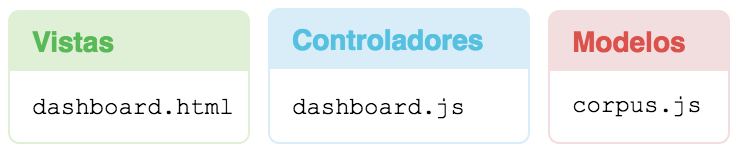
\includegraphics[width=\textwidth]{images/ui-nabu-mvc-dashboard}
    \caption{\textit{Componentes MVC de la sección Dashboard.}}
    \label{fig:ui-nabu-mvc-dashboard}
\end{figure}

\paragraph{Corpus}

En la implementación de esta sección se utilizaron dos vistas. La vista principal implementada en el
archivo \texttt{corpus-search.html} presenta el formulario de búsqueda y los resultados. Se tiene una
vista secundaria en \texttt{document-detail.html} para presentar el cuadro de diálogo con los detalles
de un documento particular.

Se utilizaron además dos controladores para la lógica de la sección. En \texttt{corpus.js} se maneja la
creación de las consultas en formato JSON, el control de la tabla de resultados y la utilización de la
biblioteca Ace~\cite{AceJS} para dibujar el cuadro de texto para las consultas avanzadas. También se cuenta
con el controlador \texttt{document-detail-dialog.js} que se encarga de controlar el cuadro de diálogo
para los detalles de los documentos. Esta sección utiliza también el servicio \texttt{corpus.js}, que ya fue
descrito en la sección anterior.

\begin{figure}[h]
    \centering
    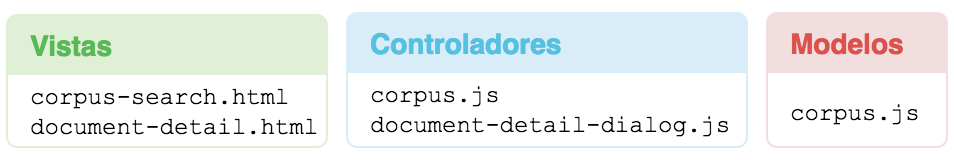
\includegraphics[width=\textwidth]{images/ui-nabu-mvc-corpus}
    \caption{\textit{Componentes MVC de la sección Corpus.}}
    \label{fig:ui-nabu-mvc-corpus}
\end{figure}

\paragraph{Embeddings}

Para la implementación de esta sección se utilizaron dos vistas principales. En el archivo
\texttt{embeddings.html} se implementa la vista con la lista de representaciones vectoriales del sistema,
mientras que en \texttt{embedding-detail.html} se encuentra el código de la vista en detalle para una
representación vectorial en particular. Se tienen además vistas adicionales para crear una nueva representación
y para evaluar las representaciones ya existentes, en los archivos \texttt{embedding-new.html} y
\texttt{evaluate-on-testset-dialog.html} respectivamente.

Desde el punto de vista lógico, se utiliza el controlador \texttt{embeddings.js} para dibujar la lista de
representaciones vectoriales y actualizar el indicador de progreso para aquellas representaciones que están
siendo entrenadas. El controlador \texttt{embedding-detail.js} es utilizado en la vista de detalles de una
representación vectorial y se encarga de construir las tablas de datos y mantener actualizado el indicador de
progreso de entrenamiento. Además, se encarga de realizar algunos procesos de formateo de los datos obtenidos
de los servicios \texttt{services/embeddings.js} y \texttt{services/jobstesting.js}, utilizados para consumir
los endpoints de representaciones vectoriales y casos de prueba, respectivamente. También se utiliza el servicio
\texttt{services/jobstraining.js} para la comunicación con los endpoints encargados de manejar el entrenamiento
de representaciones vectoriales.

Conviene destacar también el controlador \texttt{embedding-new-dialog.js} que se encarga de presentar los
datos para la creación de una nueva representación vectorial de forma eficiente y mutando los parámetros
presentados en función del algoritmo de entrenamiento seleccionado. Este controlador y su vista acompañante
pueden ser invocados desde la vista de resultados de consultas al corpus, como ya se explico en la sección
anterior.

\begin{figure}[h]
    \centering
    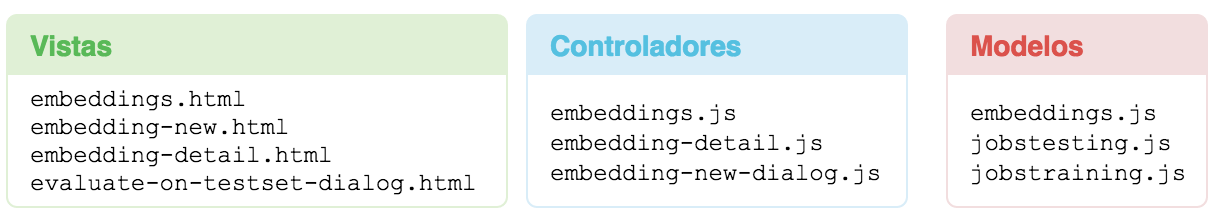
\includegraphics[width=\textwidth]{images/ui-nabu-mvc-embeddings}
    \caption{\textit{Componentes MVC de la sección Embeddings.}}
    \label{fig:ui-nabu-mvc-embeddings}
\end{figure}

\paragraph{Tests}

Como en el caso de la sección \textit{Embeddings}, para la implementación de esta sección también se
utilizaron dos vistas principales. La vista con la lista de casos de prueba del sistema fue implementada en
el archivo \texttt{tests.html}. La implementación de la vista de detalles de un caso de prueba se incluye
en el archivo \texttt{test-detail.html}. Para las demás funcionalidades se utilizaron vistas auxiliares. La
creación de nuevos casos de prueba y nuevos trabajos de evaluación fueron implementadas utilizando sendos
cuadros de diálogo implementados en \texttt{test-new.html} y \texttt{test-embedding-new.html},
respectivamente. Finalmente, la vista en detalle de los resultados de una evaluación sobre una
representación vectorial fue implementada con otro cuadro de diálogo en \texttt{test-result-dialog.html}.

Para la lógica de esta sección se utilizaron varios controladores. En la vista de listado de casos de
prueba se utilizó el controlador \texttt{tests.js}, encargado mayoritariamente de dibujar la lista y
actualizar el progreso de ejecución de los trabajos de evaluación. Para la vista de detalles se implementó
el controlador \texttt{test-detail.js}, responsable de dibujar las tablas de datos, mantener actualizadas
las barras de progreso de evaluación y llevar la cuenta de la cantidad de trabajos ejecutándose en cada
momento. Adicionalmente, el controlador \texttt{test-new-dialog.js} fue utilizado para manejar la creación
de nuevos casos de prueba. Finalmente los controladores \texttt{test-result-dialog.js} y
\texttt{new-embedding-test-dialog.js} fueron utilizados para desplegar la información detallada de la
ejecución de un caso de prueba en una representación vectorial y la creación de nuevos trabajos de
entrenamiento, respectivamente.

Los servicios más importantes para esta sección son \texttt{testsets.js} para realizar operaciones
CRUD (crear, recuperar, actualizar y destruir) sobre los casos de prueba, \texttt{results.js} para
consultar los resultados de la evaluación de representaciones vectoriales y \texttt{jobstesting.js}, para
la creación de nuevos trabajos de evaluación en el sistema.

\begin{figure}[h]
    \centering
    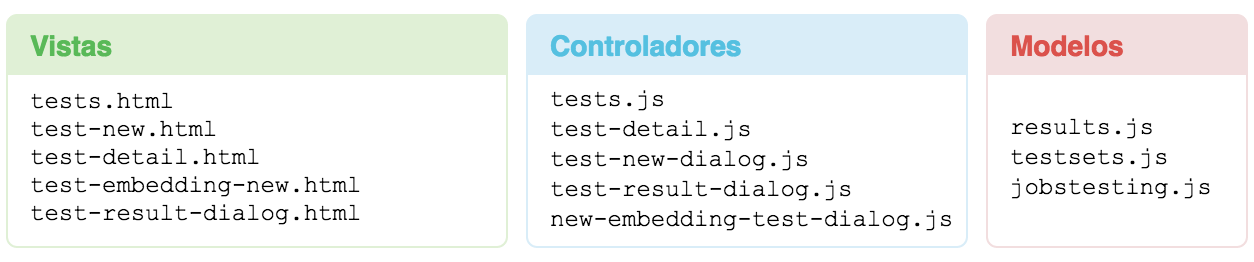
\includegraphics[width=\textwidth]{images/ui-nabu-mvc-tests}
    \caption{\textit{Componentes MVC de la sección Tests.}}
    \label{fig:ui-nabu-mvc-tests}
\end{figure}

\subsubsection{Consideraciones de diseño}

Una vez terminado el análisis de la arquitectura del frontend, es interesante mencionar ciertos objetivos y
decisiones que guiaron la construcción del mismo. Se incluye a continuación una lista de puntos que fueron
tomados en cuenta al momento de construir la solución.

\begin{itemize}

\item Desde su concepción, se buscó que el frontend sea altamente flexible ante cambios en la API expuesta
por el backend. Es decir, se buscó parametrizar la vistas más complejas de modo de soportar cambios en la
cantidad o formato de ciertos campos con el mínimo impacto en el código del frontend. Como ejemplo se tiene
la vista de creación de nuevas representaciones vectoriales. La API define un formato específico y flexible
para los parámetros de entrenamiento de un nuevo vector en función del algoritmo de entrenamiento elegido.
De esta forma se pueden agregar nuevas clases de algoritmos en el backend y estos estarán disponibles en el
frontend sin requerir modificaciones adicionales.

\item Se buscó también lograr una interfaz sencilla e intuitiva. Fue por este motivo que se decidió
utilizar el Diseño Material de Google al ser una tecnología ampliamente probada y aceptada. Principalmente
se logró presentar la información y funcionalidades de forma directa y clara pero manteniendo un estilo
consistente y elegante en todas las pantallas.

\item Se consideró como prioritario construir una interfaz rápida y eficiente que aproveche al máximo las
ventajas de los navegadores modernos. A pesar de que este proyecto no tiene como objetivo probar técnicas
de diseño y programación para la web, buscamos en todo momento lograr un desarrollo de calidad que utilice
las bondades y excelentes avances de las herramientas para la creación de aplicaciones web modernas.

\item Finalmente se puso como objetivo lograr un diseño desacoplado para la interacción de los componentes
backend y frontend de la herramienta. Esto se consiguió utilizando la API REST expuesta como único punto de
intercambio entre ambas componentes. Entre otras ventajas, esto permite eventualmente poner en producción
cada componente en nodos separados.

\end{itemize}
